% ============================================================
%  Exposición-Demostración: MDD (UML -> Código) con BOUML
%  Asignatura: Ingeniería de Requisitos (ISR-401) -- UTEQ 2026-2027 PPA
%  Sistema del PFC: MundiPets
%  Herramienta MDD: BOUML
%  Formato: IEEE onecolumn | Biber + biblatex (estilo IEEE)
% ============================================================
\documentclass[journal,onecolumn]{IEEEtran}

% ── Codificación e idioma ───────────────────────────────────
\usepackage[T1]{fontenc}
\usepackage[utf8]{inputenc}
\usepackage[spanish, es-tabla]{babel}
\usepackage[autostyle=true, spanish=mexican]{csquotes}

% ── Tablas ──────────────────────────────────────────────────
\usepackage{booktabs}
\usepackage{tabularx}
\usepackage{array}
\usepackage{multirow}
\usepackage{longtable}
\newcolumntype{C}[1]{>{\centering\arraybackslash}p{#1}}
\newcolumntype{L}[1]{>{\raggedright\arraybackslash}p{#1}}

% ── Figuras y Ajuste de Espacios en Blanco ──────────────────
\usepackage{graphicx}
\usepackage{float}
\setlength{\textfloatsep}{10pt plus 2pt minus 4pt}
\setlength{\floatsep}{8pt plus 2pt minus 2pt}
\setlength{\intextsep}{10pt plus 2pt minus 2pt}

% ── Color y enlaces ─────────────────────────────────────────
\usepackage{xcolor}

% ── Geometría ─────────────────────────────────────────────
\usepackage{geometry}
\geometry{a4paper, top=2.2cm, bottom=2.2cm, left=2.2cm, right=2.2cm, headheight=14pt, footskip=1.0cm}

% ── Encabezado ────────────────────────────────────────────
\usepackage{fancyhdr}
\pagestyle{fancy}
\fancyhf{}
\renewcommand{\headrulewidth}{0.4pt}
\fancyhead[L]{\small Ingeniería de Requisitos -- Exposición-Demostración MDD - BOUML}
\fancyhead[R]{\small MundiPets}
\fancyfoot[C]{\thepage}

% ── Espaciado y Parches ─────────────────────────────────────
\usepackage{parskip}
\setlength{\parskip}{3pt}
\makeatletter
\@ifundefined{labelindent}{}{\let\labelindent\relax}
\makeatother
\usepackage{enumitem}
\setlist{nosep} % Compactar todas las listas (itemize/enumerate)
\usepackage{caption}
\usepackage{titlesec}
\captionsetup{font=small, labelfont=bf}
\usepackage{amssymb}

% ── Forzar "Tabla" en lugar de "Cuadro" ──────────────────────
\renewcommand{\thetable}{\arabic{table}}
\def\tablename{Tabla}

% ── Compactación extrema para el Índice (Ocupar 1 página) ──
\usepackage{tocloft}
\setlength{\cftbeforesecskip}{2pt}       % Espacio antes de secciones
\setlength{\cftbeforesubsecskip}{0pt}    % Espacio antes de subsecciones
\setlength{\cftparskip}{-1pt}            % Espacio de párrafo general en TOC

% Forzar el punto después del número en el índice (Ej: 1. Marco Teórico)
\renewcommand{\cftsecaftersnum}{.}
\renewcommand{\cftsubsecaftersnum}{.}

% ── Configuración de la Caja de Código (Estilo Visual Studio / C# / C++) ──
\usepackage{listings}
\definecolor{backgroundgray}{gray}{0.95}
\definecolor{keywordblue}{rgb}{0.0, 0.0, 0.7}
\definecolor{stringpurple}{rgb}{0.5, 0.0, 0.5}
\definecolor{commentgray}{rgb}{0.4, 0.4, 0.4}
\definecolor{numbergray}{gray}{0.6}

\lstset{
	language=C++,
	backgroundcolor=\color{backgroundgray},
	basicstyle=\small\ttfamily,
	keywordstyle=\bfseries\color{keywordblue},
	stringstyle=\color{stringpurple},
	commentstyle=\itshape\color{commentgray},
	numbers=left,
	numberstyle=\tiny\color{numbergray},
	stepnumber=1,
	numbersep=10pt,
	showstringspaces=false,
	breaklines=true,
	frame=single,
	rulecolor=\color{gray!40},
	framexleftmargin=6pt,
	framexrightmargin=6pt,
	framextopmargin=6pt,
	framexbottommargin=6pt,
	xleftmargin=15pt,
	xrightmargin=15pt,
	abovecaptionskip=8pt
}

% Redefinir etiqueta para que diga "Código" en vez de "Listing"
\renewcommand{\lstlistingname}{Código}

% ── Formato de Secciones ────────────────────────────────────
\renewcommand{\thesection}{\arabic{section}}
\renewcommand{\thesubsection}{\thesection.\arabic{subsection}}
\renewcommand{\thesubsubsection}{\thesubsection.\arabic{subsubsection}}

\titleformat{\section}{\normalfont\Large\bfseries}{\thesection.}{1em}{}
\titleformat{\subsection}{\normalfont\large\bfseries}{\thesubsection.}{1em}{}
\titleformat{\subsubsection}{\normalfont\normalsize\bfseries}{\thesubsubsection.}{1em}{}

% ── Bibliografía: biblatex + biber, estilo IEEE ──────────────
\usepackage[
backend=biber,
style=ieee,
citestyle=numeric-comp,
isbn=true,
doi=true
]{biblatex}
\addbibresource{referencias.bib}

\usepackage[hidelinks,colorlinks=false]{hyperref}

% Reducción de profundidad del índice para ahorrar páginas
\setcounter{secnumdepth}{3}
\setcounter{tocdepth}{2}

\begin{document}
	
	% ============================================================
	% CARÁTULA
	% ============================================================
	\begin{titlepage}
		\centering
		
		{\large\bfseries UNIVERSIDAD TÉCNICA ESTATAL DE QUEVEDO\\[12pt]}
		
		
\includegraphics[width=0.16\textwidth]{figuras/logo_uteq.png}\\[12pt]
		
		{\large\bfseries FACULTAD DE CIENCIAS DE LA COMPUTACIÓN\\[4pt]
			CARRERA DE INGENIERÍA EN SOFTWARE}
		
		\vspace{0.8cm}
		
		{\normalsize\bfseries TEMA:}\\[4pt]
		{\normalsize GA – EXPOSICIÓN SEGUNDO CORTE: HERRAMIENTAS CASE (BOUML)}\\[4pt]
		\vspace{0.4cm}
		
		{\normalsize\bfseries ASIGNATURA:}\\[4pt]
		{\normalsize INGENIERÍA DE REQUISITOS}
		
		\vspace{0.4cm}
		
		{\normalsize\bfseries DOCENTE:}\\[4pt]
		{\normalsize ING. GLEISTON GUERRERO ULLOA, PhD.}
		
		\vspace{0.4cm}
		
		{\normalsize\bfseries INTEGRANTES:}\\[6pt]
		
		\textit{CHAVARRIA CUENCA TAHINY MEL},~CI: 0943050054,~tchavarriac@uteq.edu.ec\\
		\vspace{0.2cm}
		\textit{\textbf{MENDOZA PÁRRAGA ANDY JOHEL}},~CI: 1251401590,~amendozap9@uteq.edu.ec,~Titular PFC\\
		\vspace{0.2cm}
		\textit{SANCHEZ CORNEJO GARY ALBERTO},~CI: 1208338291,~gsanchezc6@uteq.edu.ec\\
		
		\vspace{0.4cm}
		{\normalsize\bfseries EQUIPO:}\\[4pt]
		{\normalsize H}
		
		\vspace{0.4cm}
		{\normalsize\bfseries CURSO/PARALELO:}\\[4pt]
		{\normalsize CUARTO SEMESTRE PARALELO ``B''}
		
		\vspace{0.4cm}
		{\normalsize\bfseries SISTEMA PFC:}\\[4pt]
		{\normalsize MundiPets (Titular: Andy Mendoza Párraga)}
		
		\vspace{0.4cm}
		{\normalsize\bfseries HERRAMIENTA MDD SELECCIONADA:}\\[4pt]
		{\normalsize BOUML}
		
		\vspace{0.4cm}
		\textbf{REPOSITORIO GITHUB:}\\[4pt]
		\url{https://github.com/andymendozap03/PFC-MundiPets-MDD-EquipoH-BOUML.git}
		
		\vspace{0.8cm}
		{\normalsize\bfseries QUEVEDO -- LOS RÍOS -- ECUADOR}\\[4pt]
		{\normalsize\bfseries 2026 -- 2027 PPA}
		
	\end{titlepage}
	
	\clearpage
	\begingroup
	\renewcommand{\clearpage}{} % Evita que comandos internos salten de página
	\tableofcontents
	\endgroup
	\clearpage
	
	% ============================================================
	% RESUMEN
	% ============================================================
	\section{Resumen}
	\addcontentsline{toc}{section}{Resumen}
	El presente documento evidencia la aplicación práctica del desarrollo guiado por modelos (MDD) para resolver la desincronización existente entre el diseño conceptual y la implementación en el Proyecto de Fin de Carrera (PFC) \textit{MundiPets}. Para mitigar el retrabajo y la pérdida de trazabilidad provocados por la traducción manual de requisitos, se seleccionó la herramienta CASE BOUML 7.11 frente a la alternativa analizada Modelio 5.4.1, debido a su flujo de configuración directo para la ingeniería directa. El modelado se enfocó exclusivamente en el alcance transaccional del subsistema de Gestión de Mascotas e Historial Médico, estructurando diagramas estáticos y de comportamiento bajo restricciones estrictas del metamodelo UML. Como resultado alcanzado, el modelo superó con éxito la auditoría sintáctica interna (\textit{Uml projection Done}), garantizando la consistencia estructural necesaria para generar automáticamente los artefactos físicos de código fuente orientados al backend del sistema. Esta transformación automatizada se configuró utilizando de forma nativa el lenguaje C++, produciendo archivos de cabecera (.h) e implementación (.cpp) completamente limpios, verificables y preparados para la compilación, cerrando el ciclo de trazabilidad propuesto.
	
	% ============================================================
	% 1. MARCO TEÓRICO 
	% ============================================================
	\section{Marco teórico}
	
	\subsection{Model-Driven Engineering (MDE)}
	La Model-Driven Engineering (MDE), o Ingeniería Dirigida por Modelos, constituye un paradigma de desarrollo de software en el que los modelos dejan de considerarse simples bosquejos o diagramas de documentación visual para convertirse en los artefactos centrales de todo el ciclo de vida del sistema \cite{Brambilla2017, Schmidt2006}. Bajo este enfoque, los modelos se explotan para abstraer las restricciones, reglas de negocio y comportamiento lógico del dominio con un nivel de abstracción muy superior al del código fuente tradicional \cite{Selic2003, Whittle2014}. A diferencia de los entornos low-code comerciales, MDE se caracteriza por el uso riguroso de lenguajes de modelado estandarizados, el establecimiento formal de metamodelos y el uso de trazas explícitas que aseguran la trazabilidad bidireccional entre los requisitos y la arquitectura de software generada \cite{DiRuscio2022LowCodeMDE, Bucaioni2022}.
	
	En el Proyecto de Fin de Curso (PFC) \textit{MundiPets}, este paradigma se operativiza al transformar la especificación de requisitos en un modelo conceptual sólido dentro del entorno operativo de BOUML \cite{ERSMundiPets2026, GuiaMDD2026}. Los procesos del dominio clínico, que abarcan desde el control de las hojas sanitarias hasta la gestión de perfiles biológicos de los animales, se modelan mediante estructuras jerárquicas tipadas, asegurando que el diseño resguarde una correspondencia exacta y verificable con las necesidades transaccionales declaradas para la plataforma web \cite{ERSMundiPets2026, GuiaMDD2026}.
	
	\subsection{Model-Driven Architecture (MDA)}
	La iniciativa Model-Driven Architecture (MDA), promovida por el Object Management Group (OMG), establece un marco de trabajo de ingeniería que aísla las especificaciones funcionales del negocio de las fluctuaciones de las plataformas tecnológicas subyacentes \cite{OMG2014MDA}. Para cumplir este propósito, MDA estructura el proceso de desarrollo de software dividiéndolo en tres niveles independientes de abstracción que interactúan mediante transformaciones sucesivas \cite{OMG2014MDA}:
	\begin{itemize}
		\item \textbf{CIM} (\textit{Computation Independent Model}): Captura las reglas del dominio y las necesidades del negocio de forma puramente conceptual, prescindiendo por completo de consideraciones computacionales o de sistemas.
		\item \textbf{PIM} (\textit{Platform Independent Model}): Expresa el diseño de la arquitectura, las entidades y las interconexiones del sistema de manera lógica, sin vincularse a tecnologías o frameworks concretos.
		\item \textbf{PSM} (\textit{Platform Specific Model}): Vincula el diseño formal (PIM) con los detalles técnicos, tipos primitivos y restricciones de una plataforma de despliegue específica para posibilitar su codificación \cite{Silega2022}.
	\end{itemize}
	A pesar de que la literatura industrial concentra sus esfuerzos en el análisis de la transformación técnica PIM–PSM, la transición del modelo CIM al PIM es clave, ya que es el nexo formal que traslada los requisitos de negocio atómicos hacia el primer modelo de diseño puro e independiente de la plataforma \cite{Silega2022}.
	
	\subsection{Model-Driven Development (MDD)}
	El Model-Driven Development (MDD), o Desarrollo Dirigido por Modelos, representa la aplicación práctica y automatizada de MDE durante la construcción del software, donde los modelos actúan como las entradas directas para la generación del código \cite{Brambilla2017, Selic2003}. Mediante este enfoque, los generadores automáticos procesan la estructura estática del modelo para instanciar el esqueleto de la aplicación, abatiendo tareas repetitivas de codificación, estandarizando convenciones sintácticas en el equipo de desarrollo y previniendo la inserción de errores estructurales manuales \cite{Whittle2014, Huning2021SafetyMechanisms}. La idoneidad de emplear herramientas CASE ligeras en este flujo radica en su capacidad de procesar esquemas lógicos nativos e intercambiables para derivar clases, métodos, firmas funcionales y dependencias sin ambigüedades técnicas \cite{Durai2022XMI}.
	
	Para el proyecto \textit{MundiPets}, el desarrollo guiado por modelos se concreta al traducir el diagrama de clases del bloque sanitario directamente en la estructura del backend de la aplicación \cite{GuiaMDD2026}. Las entidades del dominio (\textit{Usuario}, \textit{Mascota}, \textit{HistorialMedico}, \textit{MascotaVacuna} y \textit{EvaluacionVeterinaria}) se configuran con visibilidades y encapsulamientos específicos, permitiendo que la herramienta genere la base limpia del código y forzando al equipo a diferenciar metodológicamente las estructuras generadas por el modelo de la lógica de negocio especializada que se añade a mano \cite{ERSMundiPets2026, GuiaMDD2026}.
	
	\subsection{Transformaciones M2M}
	Las transformaciones modelo-a-modelo (M2M) toman un modelo de origen y producen un modelo destino, ambos conformes a sus respectivos metamodelos; dentro de MDA, el caso típico es el paso de un PIM a un PSM. El estándar del OMG que rige este tipo de transformación es QVT (\textit{Query/View/Transformation}) v1.3 \cite{OMG2016QVT}. No obstante, la evidencia empírica reciente indica que la adopción industrial de lenguajes de transformación dedicados (MTL) como QVT o ATL sigue siendo limitada frente a lo que cabría esperar de un estándar consolidado: el estudio de Höppner et al. \cite{Hppner2022}, basado en 56 entrevistas a investigadores y profesionales, documenta que la falta de tooling maduro y de evidencia sólida sobre sus ventajas frena su uso frente a lenguajes de propósito general.
	
	Esta brecha entre el estándar y la práctica industrial explica un patrón frecuente en las herramientas MDD: muchas no exponen una etapa M2M diferenciada ni un lenguaje de transformación independiente conforme a QVT, sino que absorben esa lógica dentro del propio generador de código, traduciendo el modelo de origen directamente a texto sin materializar un PSM intermedio como artefacto propio. Esto no invalida la distinción conceptual entre M2M y M2T: evidencia, más bien, que en la práctica ambas etapas suelen fusionarse cuando el objetivo final es la generación de código y no la interoperabilidad entre modelos.
	
	\subsection{Transformaciones M2T}
	Las transformaciones modelo-a-texto (M2T) generan artefactos textuales -código fuente, configuración o documentación- a partir de un modelo conforme a un metamodelo; el estándar OMG de referencia es MOFM2T v1.0 \cite{OMG2008MOFM2T}. Un ejemplo reciente de esta lógica se encuentra en el trabajo de Jiménez-Navajas et al. \cite{JimenezNavajas2025QuantumUML}, quienes implementan transformaciones M2T con el lenguaje EGL (\textit{Epsilon Generation Language}) para producir código Python y Qiskit a partir de modelos UML extendidos, lo que evidencia cómo un motor M2T recorre los elementos del modelo y los inyecta en plantillas parametrizadas para producir texto ejecutable.
	
	Las herramientas MDD implementan esta lógica de dos formas distintas. Por un lado, motores declarativos como Acceleo o EGL exponen la plantilla como un archivo de texto editable que sigue, con distinto grado de fidelidad, la gramática propuesta por MOFM2T. Por otro lado, un grupo amplio de herramientas comerciales integra la generación como un módulo o plug-in compilado que lee las clases, atributos, relaciones y operaciones del modelo y las vuelca en código siguiendo plantillas fijas embebidas en el propio generador, sin exponer una gramática pública ni permitir su edición directa; esta segunda variante limita la personalización a los parámetros que la propia herramienta expone.
	
	\subsection{Metamodelo}
	El metamodelo constituye la capa de abstracción que define las reglas gramaticales y la sintaxis abstracta que rige a un lenguaje de modelado; en el caso de UML, su semántica formal está especificada sobre el estándar MOF (\textit{Meta-Object Facility}) del OMG \cite{OMG2017UML}. Los generadores de código automatizados no interpretan de manera libre o visual los diagramas de un lienzo, sino que ejecutan reglas sintácticas analizando las relaciones lógicas que el metamodelo base garantiza que existen en el árbol del proyecto \cite{DiFelice2022}. La calidad y precisión de este metamodelo restringe directamente la viabilidad de la ingeniería directa, puesto que cualquier ambigüedad u omisión de tipos degrada la estructura de los artefactos generados \cite{DiRocco2022}. BOUML procesa recursivamente esta sintaxis abstracta para traducir de forma exacta las relaciones de generalización, agregación y composición hacia punteros, vectores y herencias nativas de C++ \cite{BOUMLFeatures2026}.
	
	\subsection{Perfiles UML}
	Los perfiles UML representan el mecanismo estándar diseñado por el OMG para habilitar la extensión ligera del metamodelo, adaptando el vocabulario y comportamiento genérico de UML a plataformas tecnológicas o dominios de negocio específicos sin modificar la especificación base del lenguaje \cite{OMG2017UML}. Este mecanismo opera inyectando estereotipos, restricciones semánticas y valores etiquetados que añaden una carga semántica especializada, la cual es leída por los motores de ingeniería directa para decidir qué tipo de arquitectura física inyectar en el código destino \cite{Kraas2022, Gorski2022}. Para el subsistema clínico de \textit{MundiPets}, se aplicó el estereotipo \texttt{<<Entity>>} a las clases de dominio encargadas de la persistencia (\textit{Mascota}, \textit{HistorialMedico}, \textit{Vacuna}) y \texttt{<<Actor>>} a las clases de control e interacción de usuarios, permitiendo al generador discriminar la lógica de los archivos de salida \cite{ERSMundiPets2026, BOUMLFeatures2026}.
	
	\subsection{Plantilla / template}
	Una plantilla o \textit{template} es el fragmento parametrizado que la herramienta MDD instancia por cada elemento del modelo para producir el código correspondiente. Este mecanismo puede implementarse como archivo de texto editable, ligado a una gramática de tipo MOFM2T, o puede empaquetarse como un componente compilado que aplica la definición del modelo sin exponerla como texto. Paolone et al. \cite{Paolone2021} documentan este segundo caso con xGenerator, una plataforma MDA propietaria que genera aplicaciones Java MVC completas a partir de un modelo UML sin exponer la plantilla al desarrollador, tratándola como una caja negra cuya salida solo puede evaluarse por la calidad del código resultante y no por inspección directa de la plantilla.
	
	Un mecanismo de parametrización habitual en este tipo de generadores es el bloque protegido: toda operación cuyo cuerpo se delimita mediante marcadores reservados conserva, en regeneraciones sucesivas, el contenido que el desarrollador haya escrito manualmente, evitando que una nueva ejecución del generador sobrescriba la lógica de negocio ya implementada. Este mecanismo es coherente con la lógica M2T y con el estándar MOFM2T \cite{OMG2008MOFM2T}, y constituye la base técnica que permite un ciclo de \textit{roundtrip} controlado: el modelo puede regenerarse repetidamente sin perder el trabajo manual, siempre que este se mantenga dentro de los delimitadores correspondientes.
	
	\subsection{Forward, reverse y round-trip engineering}
	La ingeniería de software bidireccional abarca tres procesos de transformación complementarios orientados a mantener la consistencia entre el diseño y los archivos físicos: el \textit{forward engineering} (ingeniería directa) automatiza la traducción de modelos abstractos a código fuente; el \textit{reverse engineering} analiza estáticamente los archivos fuente en disco para recuperar su estructura y plasmarla en diagramas UML; y el \textit{round-trip engineering} unifica ambos sentidos, gestionando la sincronización interactiva cuando cualquiera de los dos artefactos experimenta cambios evolutivos \cite{Brambilla2017, Selic2003, Kannengiesser2021}. Mantener esta paridad en entornos industriales es uno de los mayores desafíos metodológicos debido a las modificaciones concurrentes y a la inserción de código manual \cite{Jongeling2022}. En \textit{MundiPets}, el ciclo se cierra aplicando un cambio controlado en el modelo de clases, regenerando las firmas en C++ y verificando físicamente que BOUML respete el código humano embebido en sus bloques protegidos \cite{GuiaMDD2026}.
	
	\subsection{Diagramas UML admisibles como origen}
	El diagrama de clases representa el artefacto nuclear e imprescindible para la generación estructural de código fuente dentro del paradigma MDD, relegando a vistas de comportamiento o interacción a un rol estrictamente complementario \cite{Brambilla2017}. Esta jerarquía teórica se convalida plenamente con la evidencia empírica industrial: encuestas globales reflejan que el diagrama de clases es la primera opción elegida unánimemente por los desarrolladores para modelar la estructura funcional (71\%) y la arquitectura de datos (85\%) de los sistemas complejos, demostrando que centrar la ingeniería directa en esta vista estática responde a la práctica dominante del desarrollo corporativo \cite{Ozkaya2020}. En concordancia con este alcance, el módulo de gestión sanitaria de \textit{MundiPets} se modeló explotando esta perspectiva estructural de tipos y herencias, integrándose de forma nativa con el diagrama de casos de uso para delimitar las fronteras de interacción de los actores en BOUML \cite{GuiaMDD2026}.
	
	\subsection{Estado del arte}
	En la actualidad, la Ingeniería Dirigida por Modelos ha evolucionado hacia la confluencia con lenguajes específicos de dominio (DSL), plataformas low-code avanzadas y flujos de automatización integrados en arquitecturas DevOps \cite{Alharbi2026AutomaticCodeGeneration, Lehner2025}. A pesar de estos avances, persisten desafíos de investigación abiertos en torno a la escalabilidad de las transformaciones M2M complejos, la preservación a largo plazo de mapas de trazabilidad multidimensionales y la sincronización continua entre el diseño gráfico y la implementación física \cite{Kahani2019, Jongeling2022}. En este panorama, herramientas CASE ligeras y robustas como BOUML 7.11 demuestran su vigencia al proveer un entorno óptimo para la ingeniería estructural, abstrayendo la complejidad de la codificación repetitiva, garantizando compilaciones nativas limpias y certificando un nexo auditable entre los requisitos atómicos de la ingeniería de requisitos y el software final en C++ \cite{BOUML2025, GuiaMDD2026}.
	
	% ============================================================
	% 2. JUSTIFICACIÓN DE LA SELECCIÓN DE LA HERRAMIENTA
	% ============================================================
	\section{Justificación de la selección de BOUML}
	
	\subsection{Herramienta seleccionada y versión}
	La herramienta seleccionada para desarrollar la demostración de Ingeniería Dirigida por Modelos (MDD) aplicada al PFC \textit{MundiPets} es BOUML 7.11, parche 4 \cite{BOUML2025}. Esta versión fue escogida por ofrecer un entorno UML optimizado y de alto rendimiento orientado al modelado estructural, la generación automática de código, la ingeniería inversa y el \textit{round-trip engineering} \cite{BOUMLFeatures2026}. BOUML es una herramienta UML 2 de uso gratuito y multiplataforma, con soporte nativo para diferentes lenguajes de programación estructurados y orientados a objetos, entre los cuales se destaca C++ debido a su eficiencia en la administración física de la memoria del backend \cite{BOUML2025, BOUMLFeatures2026}.
	
	Para la ejecución práctica del proyecto, se configuró C++ como el lenguaje objetivo central. BOUML se empleará para construir el diagrama de clases y de casos de uso del subsistema sanitario, transformando el diseño conceptual directo en archivos físicos de implementación base (.h y .cpp) \cite{BOUMLFeatures2026}. El alcance operativo del entorno CASE se concentrará estrictamente en los elementos derivados de forma directa del metamodelo UML, delegando la capa de persistencia SQL, las interfaces gráficas y las reglas del negocio específicas a una fase complementaria de desarrollo manual \cite{ERSMundiPets2026}. La versión seleccionada garantiza un entorno libre de errores sintácticos y reproducible, permitiendo que cualquier integrante del equipo pueda regenerar el código fuentes con las mismas marcas arquitectónicas en cualquier estación de trabajo \cite{GuiaMDD2026}.
	
	\subsection{Justificación frente a los requisitos del PFC}
	La selección de BOUML se justificó analizando las restricciones funcionales de \textit{MundiPets}, la arquitectura modular planteada en la ERS y la obligatoriedad de demostrar la trazabilidad modelo-código en la evaluación académica \cite{GuiaMDD2026, ERSMundiPets2026}.
	\begin{itemize}
		\item \textbf{Correspondencia con el dominio modelado:} El subsistema clínico puede estructurarse limpiamente mediante clases del negocio como \textit{Usuario}, \textit{Mascota}, \textit{HistorialMedico}, \textit{Vacuna}, \textit{MascotaVacuna} y \textit{EvaluacionVeterinaria} \cite{ERSMundiPets2026}. BOUML permite tipificar atributos primitivos, firmas de operaciones públicos/protegidos y cardinalidades complejas, resolviendo la lógica estática del dominio sin ambigüedades técnicas \cite{BOUMLFeatures2026}.
		\item \textbf{Generación eficiente de código backend:} La herramienta automatiza la traducción estructural, reduciendo la escritura manual redundante y garantizando que las asociaciones (como la composición fuerte mascota-historial) se transformen en punteros y vectores fuertemente tipados bajo el estándar de C++ \cite{BOUMLFeatures2026}. Esto disminuye el retrabajo metodológico y formaliza las bases de la aplicación \cite{Durai2022XMI}.
		\item \textbf{Arquitectura modular y encapsulamiento:} La ERS de \textit{MundiPets} exige un sistema desacoplado para integrar dinámicamente futuros componentes como módulos de inteligencia artificial o pasarelas de adopción \cite{ERSMundiPets2026}. En BOUML, las clases se organizan mediante paquetes lógicos y vistas conceptuales separadas del Browser, forzando la separación inicial de responsabilidades y un control estricto de visibilidades \cite{BOUMLFeatures2026}.
		\item \textbf{Trazabilidad en el cierre del ciclo (Round-trip):} La herramienta cumple de manera nativa con la restricción académica de inyectar cambios controlados en el diagrama (como la inserción de nuevos atributos o métodos), regenerar los archivos físicos y verificar visualmente que las firmas se actualicen en los fuentes sin corromper la lógica programada a mano en sus bloques protegidos \cite{BOUMLFeatures2026, GuiaMDD2026}.
		\item \textbf{Licencia y curva de aprendizaje:} Al ser un software de uso gratuito y consumo ligero de recursos físicos, optimiza el trabajo concurrente del equipo sin requerir inversiones comerciales \cite{BOUML2025}. Su interfaz compacta permite focalizar la atención en la consistencia de los diagramas, la parametrización de plantillas y el éxito de la compilación directa \cite{BOUMLFeatures2026}.
	\end{itemize}
	
	\subsection{Comparación con alternativa descartada}
	La alternativa de código abierto analizada por el equipo fue Modelio 5.4.1, la cual admite el modelado de múltiples lenguajes y estándares de arquitectura como BPMN, ArchiMate y SysML mediante la adición de extensiones modulares \cite{Modelio2026}. Si bien Modelio posee robustez corporativa, fue descartada formalmente debido a que la sobrecarga en la configuración de sus módulos de generación Java/C++ y su pesada interfaz gráfica excedían el alcance inmediato exigido para la demostración transaccional de \textit{MundiPets} \cite{GuiaMDD2026}. Para los objetivos académicos planteados, BOUML ofrece un flujo de trabajo significativamente más directo, un motor de ingeniería directa integrado de forma nativa en la raíz del proyecto y una menor fricción técnica para validar la consistencia del código generado \cite{BOUMLFeatures2026, GuiaMDD2026}.
	
	\begin{table}[H]
		\caption{Comparación técnica entre BOUML y la alternativa descartada Modelio.}
		\label{tab:comparacion_herramientas}
		\centering
		\renewcommand{\arraystretch}{1.2}
		\begin{tabularx}{\linewidth}{|l|X|X|X|}
			\hline
			\textbf{Criterio} & \textbf{BOUML 7.11 (Parche 4)} & \textbf{Modelio 5.4.1} & \textbf{Decisión para MundiPets} \\
			\hline
			\textbf{Licencia y Costo} & Uso gratuito; no requiere licencias comerciales \cite{BOUML2025}. & Código abierto sin costos de activación \cite{Modelio2026}. & Ambos cumplen gratuidad académica \cite{GuiaMDD2026}. \\ \hline
			\textbf{Generación C++} & Motor nativo integrado; mapeo directo a pares .h y .cpp \cite{BOUMLFeatures2026}. & Requiere instalación de módulos externos. & Flujo directo y limpio hacia C++ en BOUML \cite{BOUMLFeatures2026}. \\ \hline
			\textbf{Alcance Funcional} & Entorno concentrado en estándar UML e ingeniería bidireccional \cite{BOUMLFeatures2026}. & Ecosistema extenso que abarca BPMN y ArchiMate \cite{Modelio2026}. & Capacidades extras de Modelio no requeridas \cite{GuiaMDD2026}. \\ \hline
			\textbf{Configuración} & Parametrización desde la raíz del proyecto \cite{BOUMLFeatures2026}. & Exige activar módulos por separado \cite{Modelio2026}. & BOUML reduce componentes críticos a configurar \cite{GuiaMDD2026}. \\ \hline
			\textbf{Evolución y Ciclo} & Prioriza estabilidad del metamodelo y bloques protegidos \cite{BOUMLFeatures2026}. & Orientado a modelado empresarial continuo \cite{Modelio2026}. & BOUML ofrece relación más directa para verificación \cite{GuiaMDD2026}. \\
			\hline
		\end{tabularx}
	\end{table}
	
	% ============================================================
	% 3. DESCRIPCIÓN DEL SUBSISTEMA DEL PFC MODELADO
	% ============================================================
	\section{Descripción del subsistema del PFC modelado}
	
	\subsection{Contexto de MundiPets}
	MundiPets se constituye como una plataforma digital integral orientada a facilitar y organizar los procesos de adopción y cruza responsable de mascotas, respondiendo a la necesidad de contar con un canal centralizado, transparente y seguro. El sistema actúa como un nodo de conexión entre diversos actores clave, incluyendo propietarios de mascotas, adoptantes, interesados en cruza, refugios de animales y veterinarias.
	
	A través de esta plataforma, se busca centralizar y digitalizar la gestión de perfiles biológicos de los animales, el almacenamiento de historiales clínicos, la publicación de anuncios y la verificación de certificados. De este modo, MundiPets organiza de manera eficiente la interacción entre los usuarios que desean dar o recibir una mascota en custodia, aquellos que buscan un emparejamiento biológico controlado para sus ejemplares, y los profesionales veterinarios encargados de avalar la veracidad sanitaria de la información registrada.
	
	\subsection{Módulo seleccionado}
	El componente del sistema seleccionado para trabajar en la herramienta corresponde al subsistema de Gestión de Mascotas e Historial Médico de MundiPets. Este bloque operativo es fundamental, ya que se encarga de administrar toda la información básica, clínica y de control de los animales antes de habilitar otros procesos dentro de la plataforma.
	
	De acuerdo con el diagrama del sistema, el módulo está conformado por un conjunto interconectado de clases que organizan el dominio: la clase base \textit{Usuario} junto con sus herencias específicas (\textit{Propietario} y \textit{Veterinario}), la entidad central \textit{Mascota}, el \textit{HistorialMedico} (vinculado mediante una relación de composición rígida), el catálogo de \textit{Vacuna}, la clase asociativa \textit{MascotaVacuna} (que resuelve el carné sanitario) y la entidad \textit{EvaluacionVeterinaria} para registrar las revisiones de salud. A través de estas clases, el subsistema permite registrar los datos generales de los animales, almacenar antecedentes clínicos, controlar las dosis de vacunas aplicadas y gestionar las evaluaciones profesionales correspondientes.
	
	\subsection{Actores}
	Los actores que interactúan de forma directa con el subsistema seleccionado se definen a partir de los roles representados en la jerarquía del modelo UML:
	\begin{itemize}[leftmargin=*]
		\item \textbf{Propietario:} Es el usuario que registra y administra a los animales dentro de la plataforma. Sus acciones principales incluyen ingresar la información general de la mascota, actualizar sus datos básicos, registrar antecedentes médicos iniciales y gestionar sus publicaciones en el sistema.
		\item \textbf{Veterinario:} Es el actor profesional encargado de auditar la información de salud. Sus funciones dentro de este módulo abarcan la validación de los historiales clínicos, la carga y revisión de documentos oficiales de respaldo, y el registro de las evaluaciones veterinarias correspondientes.
	\end{itemize}
	
	\subsection{Requisitos funcionales}
	El alcance del subsistema modelado comprende las operaciones de registro, actualización, consulta y validación profesional de la información biológica y clínica de los animales. Los requisitos funcionales específicos que rigen este módulo se detallan a continuación:
	
	\begin{table}[H]
		\caption{Requisitos funcionales del subsistema de Gestión de Mascotas e Historial Médico.}
		\label{tab:rf_modulo}
		\centering
		\renewcommand{\arraystretch}{1.2}
		\begin{tabularx}{\linewidth}{|l|l|X|}
			\hline
			\textbf{ID} & \textbf{Requisito} & \textbf{Descripción} \\
			\hline
			\textbf{RF-01} & Registrar mascota & El sistema deberá permitir al propietario registrar una mascota ingresando su información general, incluyendo nombre, especie, raza, sexo, edad, estado reproductivo y fotografías para su identificación dentro de la plataforma. \\ \hline
			\textbf{RF-02} & Gestionar historial médico & El sistema deberá permitir registrar y actualizar el historial médico de una mascota, incluyendo vacunas, desparasitaciones, enfermedades, alergias, cirugías, tratamientos y controles veterinarios. \\ \hline
			\textbf{RF-03} & Consultar perfil completo & El sistema deberá permitir visualizar el perfil completo de una mascota mostrando su información general, historial médico autorizado, fotografías, comportamiento, vacunas, edad, raza para procesos de adopción o cruza. \\ \hline
			\textbf{RF-09} & Validar información médica & El sistema deberá permitir que una veterinaria autorizada valide la información médica registrada de una mascota, indicando que los datos han sido verificados por un profesional. \\ \hline
			\textbf{RF-14} & Gestionar carnet de vacunación & El sistema deberá permitir registrar, actualizar y consultar el carnet de vacunación de cada mascota, mostrando el historial de vacunas aplicadas, fechas, próximas dosis y su estado de vigencia. \\ \hline
			\textbf{RF-16} & Gestionar antecedentes genéticos & El sistema deberá permitir registrar y consultar los antecedentes genéticos y el grado de parentesco de una mascota, incluyendo información sobre enfermedades hereditarias y linaje para apoyar los procesos de cruza responsable y la evaluación de compatibilidad. \\
			\hline
		\end{tabularx}
	\end{table}
	La documentación detallada con la caracterización completa de los ocho atributos de gestión y la especificación atómica de cada uno de estos requisitos funcionales se encuentra recopilada de manera íntegra en el \textbf{Anexo A}.
	
	\subsection{Alcance del módulo modelado}
	El alcance del trabajo con la herramienta se enfoca exclusivamente en la definición de la estructura estática del subsistema de mascotas e historial médico, estableciendo los límites de lo que se incluye y lo que se excluye en este proceso:
	
	\textbf{Elementos incluidos dentro del alcance:}
	\begin{itemize}[leftmargin=*]
		\item Definición visual de las clases involucradas con sus respectivos nombres, atributos tipificados (como \textit{string} o \textit{long}) y firmas de métodos públicos o privados.
		\item Representación de las relaciones UML del dominio, incluyendo la generalización (herencia), la composición fuerte entre la mascota y su historial, y las asociaciones con multiplicidades.
		\item Modelado de la estructura de las relaciones complejas mediante el uso de clases asociativas dedicadas, como es el caso del control del carné de vacunación.
	\end{itemize}
	
	\textbf{Elementos excluidos del alcance:}
	\begin{itemize}[leftmargin=*]
		\item El desarrollo de la lógica interna o programación detallada del cuerpo de los métodos y funciones del negocio.
		\item La configuración física de esquemas, tablas o conexiones de bases de datos.
		\item El diseño visual o maquetado de las pantallas de la interfaz gráfica del usuario.
	\end{itemize}
	
	% ============================================================
	% 4. MODELO UML DE ORIGEN
	% ============================================================
	\section{Modelo UML de origen}
	En esta sección se detalla la estructuración, las características técnicas y las restricciones semánticas del modelo UML desarrollado directamente dentro del entorno operativo de BOUML. Este modelo consolida la lógica del negocio para el subsistema de Gestión de Mascotas e Historial Médico de MundiPets, sirviendo como la fuente de datos autoritativa y estructurada para el proceso posterior de ingeniería directa y generación automática de código fuente.
	
	\subsection{Diagrama de clases}
	El diagrama de clases estructural del subsistema sanitario se construyó y normalizó de manera nativa en BOUML, adaptando las especificaciones del dominio a la sintaxis del metamodelo. En la Figura \ref{fig:bouml_clases} se expone el lienzo de trabajo final, el cual integra la totalidad de los compartimentos de atributos, operaciones y visibilidades requeridos para la correcta compilación del sistema.
	
	\begin{figure}[H]
		\centering
		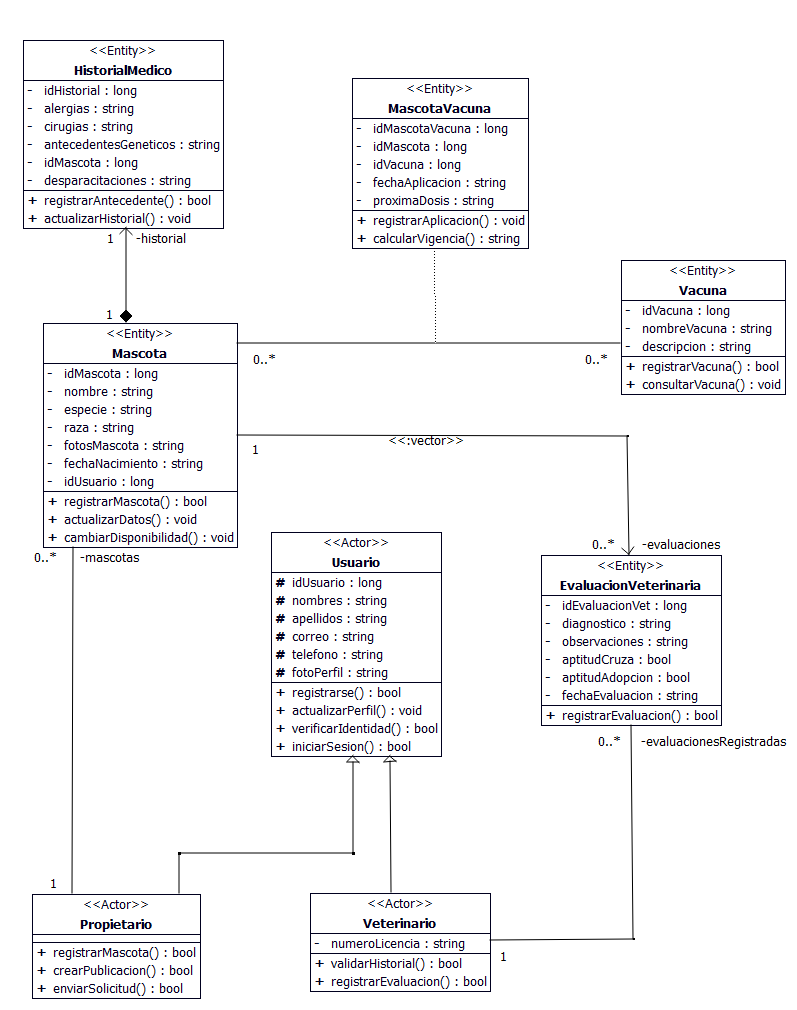
\includegraphics[width=1\textwidth]{figuras/Diagrama_ClasesSubsistema_MundiPets.png}
		\caption{Diagrama de clases del subsistema sanitario refinado en el entorno de BOUML.}
		\label{fig:bouml_clases}
	\end{figure}
	
	\newpage
	
	\subsection{Relaciones UML}
	Las conexiones que trazamos en el lienzo de BOUML dictan las reglas del negocio y definen cómo se van a comportar los punteros y contenedores en el código de C++. En la Tabla \ref{tab:clases_bouml} desglosamos detalladamente qué significa cada multiplicidad y tipo de enlazado en nuestro diseño.
	
	\begin{table}[H]
		\caption{Especificación de relaciones y multiplicidades del modelo en BOUML.}
		\label{tab:clases_bouml}
		\centering
		\renewcommand{\arraystretch}{1.1}
		\begin{tabular}{|p{3.8cm}|p{2.6cm}|p{8.2cm}|}
			\hline
			\textbf{Clases Involucradas} & \textbf{Tipo de Relación} & \textbf{Descripción de la Restricción UML} \\
			\hline
			\textit{Usuario} $\leftarrow$ \textit{Propietario} & Generalización & Herencia pura. La clase Propietario hereda y especializa los atributos del Usuario base. \\ \hline
			\textit{Usuario} $\leftarrow$ \textit{Veterinario} & Generalización & Herencia pura. La clase Veterinario extiende al Usuario común, añadiendo su licencia profesional. \\ \hline
			\textit{Mascota} $\blacklozenge$ $\rightarrow$ \textit{HistorialMedico} & Composición & Relación de existencia fuerte (1:1). El HistorialMedico depende totalmente de que exista la Mascota. \\ \hline
			\textit{Propietario} (1) $\leftrightarrow$ \textit{Mascota} (0..*) & Asociación Simple & Navegabilidad que define la propiedad. Un dueño administra de cero a muchas mascotas en su cuenta. \\ \hline
			\textit{Mascota} (*) $\leftrightarrow$ \textit{Vacuna} (*) & Clase Asociativa & Relación muchos a muchos (M:N) del estándar UML, mapeando vacunas aplicadas del catálogo. \\ \hline
			\textit{Mascota} (1) $\leftrightarrow$ \textit{MascotaVacuna} (*) & Vínculo Instancia & Conexión estructural que une a una mascota específica con las dosis de su carné sanitario. \\ \hline
			\textit{Vacuna} (1) $\leftrightarrow$ \textit{MascotaVacuna} (*) & Vínculo Catálogo & Conexión que asocia el registro de la dosis aplicada con las especificaciones de la vacuna base. \\ \hline
			\textit{Mascota} (1) $\rightarrow$ \textit{EvaluacionVeterinaria} (0..*) & Asociación Unidireccional & Define el flujo de revisiones. Una mascota acumula un historial de evaluaciones clínicas mediante un vector. \\ \hline
			\textit{Veterinario} (1) $\leftrightarrow$ \textit{EvaluacionVeterinaria} (0..*) & Asociación Simple & Vincula la responsabilidad clínica. Un veterinario es el encargado de registrar múltiples evaluaciones. \\
			\hline
		\end{tabular}
	\end{table}
	
	\subsection{Estereotipos}
	Para que el diagrama no sea solo un montón de cajas y el generador de BOUML entienda qué función cumple cada clase en la vida real, les asignamos marcas especiales llamadas \textit{estereotipos}. En el diseño del sistema usamos dos tipos principales que nos ayudan a separar los roles de los usuarios de los datos puros del negocio:
	\begin{itemize}
		\item \textbf{\texttt{<<Actor>>}:} Identifica las clases que representan a personas o roles que van a interactuar directamente con el sistema: la clase base \textit{Usuario} y sus herencias directas \textit{Propietario} y \textit{Veterinario}.
		\item \textbf{\texttt{<<Entity>>}:} Aplicado a todas las clases encargadas de almacenar y hacer persistir la información clave de la clínica veterinaria: \textit{Mascota}, \textit{HistorialMedico}, \textit{Vacuna}, la clase puente \textit{MascotaVacuna} y \textit{EvaluacionVeterinaria}.
	\end{itemize}
	
	\subsection{Atributos y operaciones tipificados}
	Para que la traducción del diagrama al código de C++ sea exacta y no genere errores al compilar, nos aseguramos de que cada atributo y método en BOUML tenga su tipo de dato bien definido. No dejamos ninguna variable al aire, sino que mapeamos todo según las necesidades reales del software:
	\begin{itemize}
		\item \textbf{Identificadores únicos (\texttt{long}):} Todas las llaves primarias del sistema (como \textit{idMascota}, \textit{idHistorial} o \textit{idUsuario}) se configuraron como de tipo \texttt{long} para garantizar escalabilidad.
		\item \textbf{Cadenas de texto (\texttt{string}):} Las variables destinadas a guardar palabras (nombres, correos, razas) se tipificaron como \texttt{string}. Se ocultó el prefijo estándar \texttt{std::} en el lienzo gráfico para mantenerlo limpio.
		\item \textbf{Métodos y operaciones (\texttt{bool} / \texttt{void}):} Las funciones que realizan controles o validaciones devuelven un tipo lógico \texttt{bool} para conocer su éxito, mientras que las destinadas únicamente a actualizar datos se configuraron con tipo de retorno \texttt{void}.
	\end{itemize}
	
	\subsection{Diagramas complementarios}
	Para complementar la perspectiva estática que nos dio el diagrama de clases, es fundamental analizar el comportamiento del sistema desde el punto de vista del usuario. Mientras que las clases definen la estructura interna, las variables y los métodos del código, los diagramas de comportamiento nos permiten entender el alcance funcional del software y qué acciones reales pueden ejecutar los actores sobre el sistema.
	
	Para este propósito, construimos un Diagrama de Casos de Uso de manera centralizada y nativa dentro del entorno de BOUML, enfocándonos exclusivamente en el alcance transaccional del subsistema de Gestión de Mascotas e Historial Médico. En este modelo se delimitan las fronteras del módulo (representadas por el recuadro del límite del sistema) y se detalla cómo los actores disparan los flujos principales:
	\begin{itemize}
		\item \textbf{Propietario:} Interactúa directamente con el subsistema activando los casos de uso destinados al registro de sus mascotas, la configuración de la privacidad médica de los datos y la consulta del perfil médico. Asimismo, maneja el registro del historial médico, flujo que cuenta con una relación de extensión (\texttt{<<extend>>}) hacia el caso de uso \textit{Cargar documento veterinario}, indicando que el usuario tiene la opción opcional de adjuntar archivos de soporte durante este proceso.
		\item \textbf{Veterinario:} Domina el flujo técnico e institucional de la clínica, teniendo acceso a la consulta del perfil médico de los pacientes y siendo el único actor encargado de disparar el caso de uso para validar la información médica en el sistema.
	\end{itemize}
	
	El desarrollo de este diagrama de comportamiento dentro de la misma herramienta de origen garantiza una coherencia absoluta en nuestro informe, demostrando que cada caso de uso del negocio cuenta con una correspondencia directa en una clase, un método y un atributo tipificado listo para soportar su ejecución en el código real de C++.
	
	\begin{figure}[H]
		\centering
		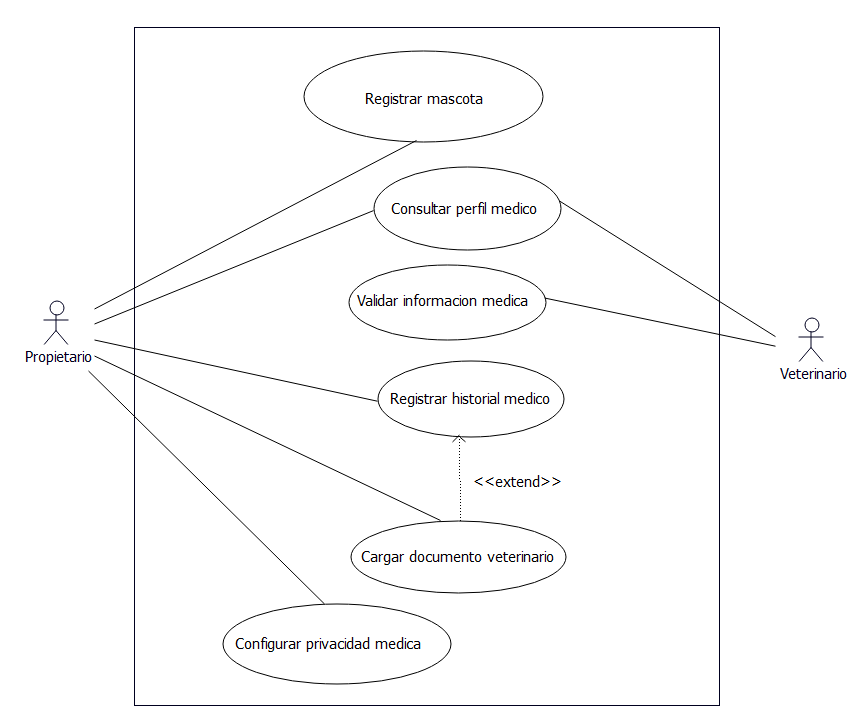
\includegraphics[width=0.72\textwidth]{figuras/Diagrama_CasosUso_Subsistema_MundiPets.png}
		\caption{Diagrama de casos de uso del subsistema sanitario desarrollado nativamente en BOUML.}
		\label{fig:casos_uso_mundipets}
	\end{figure}
	
	\subsection{Validación del modelo en BOUML}
	Antes de dar el paso definitivo hacia la ingeniería directa y generar el código fuente en C++, sometimos todo el diseño del subsistema a la herramienta de auditoría e inspección interna de BOUML. A diferencia de otros programas que son simples herramientas de dibujo genérico, BOUML cuenta con un analizador sintáctico que comprueba activamente que se cumplan las restricciones reales del metamodelo UML.
	
	Para realizar esta verificación, ejecutamos el control de consistencia jerárquica sobre el árbol del proyecto mediante la herramienta \textit{Uml projection}, monitoreando su comportamiento a través de la consola de trazas. El diagnóstico determinó que nuestro modelo está completamente limpio y libre de errores estructurales, finalizando con un estado exitoso y sin advertencias, tal como se evidencia en la Figura \ref{fig:validacion_bouml}.
	
	\begin{figure}[H]
		\centering
		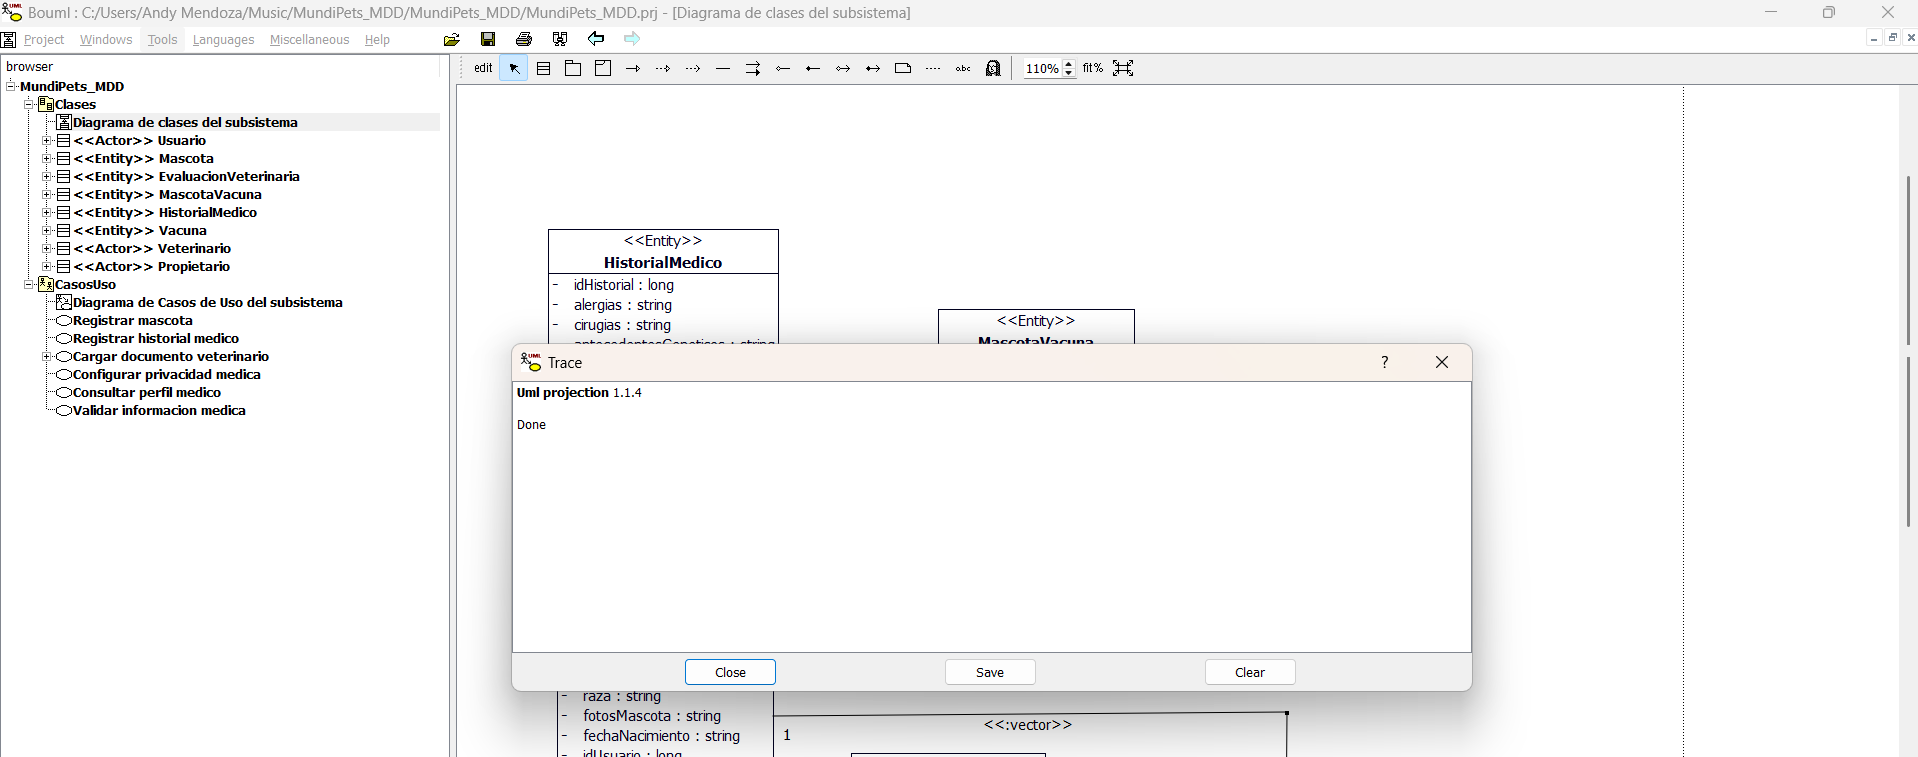
\includegraphics[width=0.62\textwidth]{figuras/Trace_Validacion_BOUML.png}
		\caption{Consola de trazas de BOUML confirmando la validación exitosa del proyecto (Uml projection Done).}
		\label{fig:validacion_bouml}
	\end{figure}
	
	Durante este proceso automatizado, el entorno validó los siguientes puntos clave del diseño:
	\begin{itemize}
		\item \textbf{Consistencia en las relaciones:} Se comprobó que todas las asociaciones, herencias, composiciones y la clase asociativa interconectan extremos bien definidos, con multiplicidades válidas que el generador puede traducir sin ambigüedades.
		\item \textbf{Integridad de tipos:} Se verificó que ninguna variable o método quedara con tipos de datos "huérfanos" o indefinidos, asegurando que los primitivos (\texttt{string}, \texttt{long}, \texttt{bool}, \texttt{void}) estén correctamente mapeados.
		\item \textbf{Validación de herencia y visibilidades:} El analizador confirmó que la jerarquía de generalización desde la clase base \textit{Usuario} hacia \textit{Propietario} y \textit{Veterinario} respeta las reglas de encapsulamiento y el acceso a los atributos protegidos (\texttt{\#}).
	\end{itemize}
	
	% ============================================================
	% 5. CONFIGURACIÓN DEL GENERADOR
	% ============================================================
	\section{Configuración del generador}
	
	\subsection{Plantilla y parámetros}
	Para transformar el diagrama de clases validado en la Sección 4 en artefactos de implementación, se utilizó el generador \textbf{C++} integrado de BOUML (versión 7.11 patch 4). En la pestaña \textit{Directory} del cuadro de diálogo \textit{Generation settings}, se estableció el directorio raíz de generación C++ (\textit{C++ root dir}) apuntando a la carpeta generado/ dentro del proyecto. En la pestaña \textit{C++[1]} se confirmaron los parámetros base: extensión de cabecera h y de implementación cpp; directivas \#include sin ruta; e indentación de 2 espacios para miembros y clases amigas, y 4 espacios para clases anidadas, junto con las guardas de inclusión automáticas (\#ifndef/\#define/\#endif) y las plantillas de cabecera e implementación.
	
	Adicionalmente, la pestaña \textit{C++[5]} reveló que BOUML resuelve los tipos contenedores externos (vector, list, map, string) mediante una tabla de correspondencia que agrega automáticamente su directiva \#include correspondiente junto con using namespace std;, por lo que el código generado referencia estos tipos sin el prefijo std:: explícito. La Figura \ref{fig:bouml_config} documenta esta configuración.
	
	\begin{figure}[H]
		\centering
		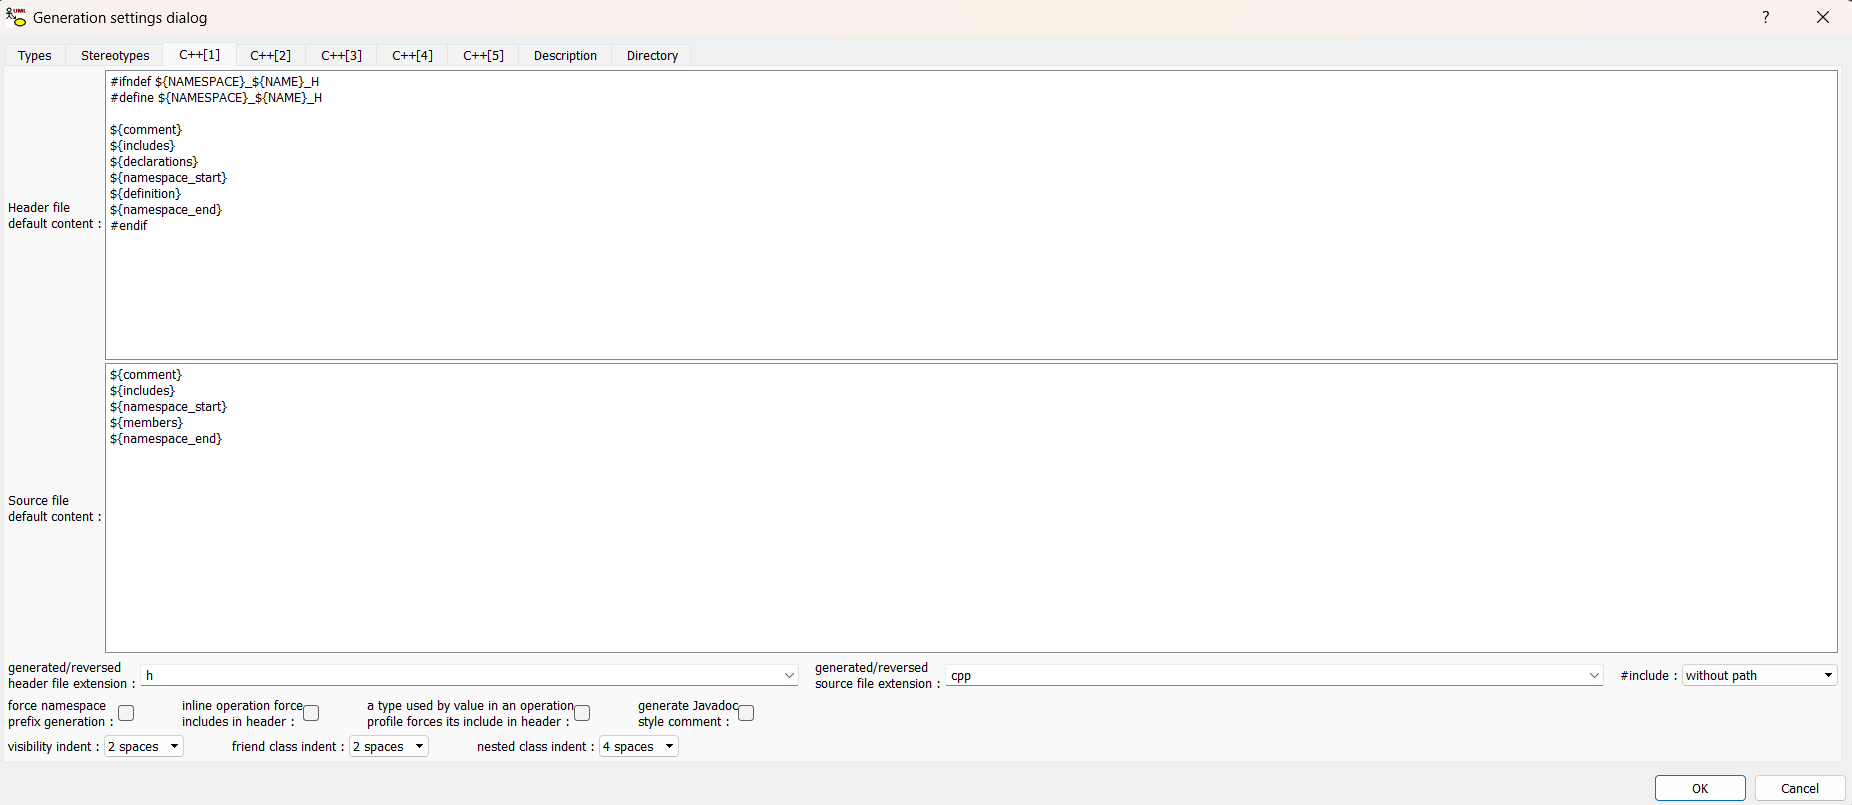
\includegraphics[width=0.72\textwidth]{figuras/bouml_config_generador.png}
		\caption{Configuración del generador C++ en BOUML: extensiones de archivo (C++[1]) y resolución de tipos externos con using namespace std; (C++[5]).}
		\label{fig:bouml_config}
	\end{figure}
	
	\subsection{Política de regeneración y decisiones de mapeo}
	La pestaña \textit{C++[3]} del generador confirmó las plantillas exactas que BOUML aplica según el tipo de relación: un atributo simple se declara como \${type} \${name}\${value};, mientras que las relaciones de asociación, agregación y composición con multiplicidad múltiple (*) se declaran anteponiendo un asterisco al nombre (\${type} * \${name}\${value};), es decir, mediante un puntero simple y no mediante un contenedor STL por defecto. Se evaluó la posibilidad de sustituir esta plantilla nativa por el tipo contenedor \texttt{vector} definido en la pestaña \textit{C++[5]} (que ya incluye su \#include <vector> y using namespace std; correspondientes) para las asociaciones con multiplicidad múltiple, como \textit{Propietario} (1) $\leftrightarrow$ \textit{Mascota} (0..*). Sin embargo, para mantener fiel el criterio de trazabilidad directa con la plantilla auditada por BOUML, el equipo decidió conservar la plantilla nativa de puntero simple sin modificarla; en consecuencia, en el código final generado \textbf{todas las asociaciones con multiplicidad múltiple se representan mediante un puntero simple} (\texttt{Mascota * mascotas;} en Propietario.h, \texttt{EvaluacionVeterinaria * evaluaciones;} en Mascota.h, etc.), y no mediante contenedores \texttt{vector}. Esta decisión implica una limitación funcional real: un puntero simple solo puede referenciar un elemento a la vez, por lo que la navegación 1--N declarada en el modelo no queda completamente representada en el código físico; esta discrepancia se documenta como limitación en la Sección 7.3. Las operaciones de acceso (\textit{getters}/\textit{setters}) se generaron siguiendo la plantilla de la pestaña \textit{C++[4]}: los métodos get\_\${name} se generan públicos, inline y const, mientras que los set\_\${name} se generan públicos sin modificadores adicionales; sin embargo, BOUML no genera estas operaciones automáticamente por defecto para los atributos del modelo (ver limitaciones, Sección 7.3), por lo que no se aplicaron sobre el código final entregado.
	
	% ============================================================
	% 6. PROCESO DE GENERACIÓN
	% ============================================================
	\section{Proceso de generación}
	
	\subsection{Ejecución y captura}
	La generación de código se ejecutó mediante la opción \textit{Generate → C++} del menú contextual sobre el paquete raíz \textit{modelo}, una vez confirmada la configuración descrita en la Sección 5.1. La consola de trazas de BOUML (\textit{Trace}) reportó el uso del \textbf{C++ generator release 5.4} y confirmó el resultado \textit{Generation done: 0 warnings, 0 errors}, evidenciando que las ocho clases del modelo (\textit{Usuario}, \textit{Propietario}, \textit{Veterinario}, \textit{Mascota}, \textit{HistorialMedico}, \textit{Vacuna}, \textit{MascotaVacuna} y \textit{EvaluacionVeterinaria}) se procesaron correctamente, produciendo dieciséis archivos —un par \texttt{.h}/\texttt{.cpp} por cada clase— sin errores ni advertencias, tal como se evidencia en la Figura \ref{fig:log_generacion}. Dado el tamaño reducido del subsistema modelado, la generación se completó de forma prácticamente instantánea (menos de un segundo), sin que la consola de trazas reporte un cronómetro explícito para esta operación.
	
	\begin{figure}[H]
		\centering
		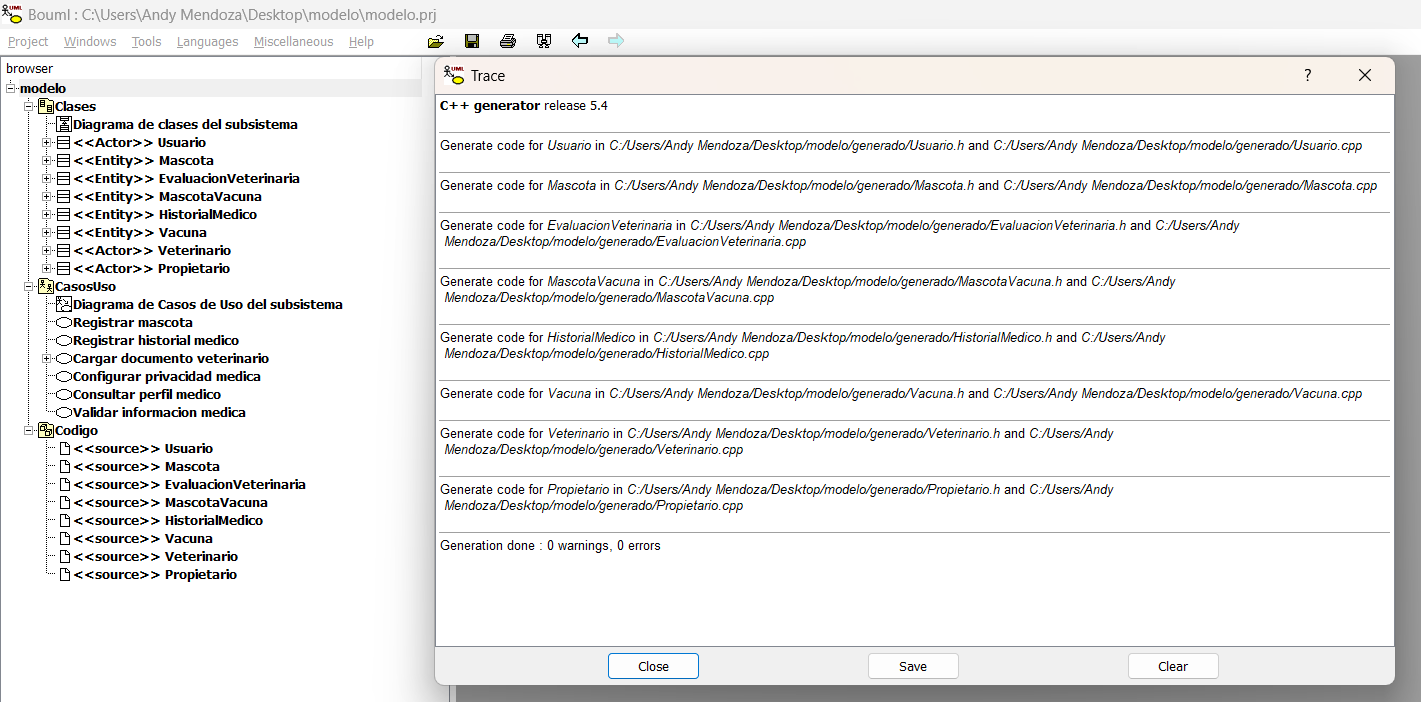
\includegraphics[width=0.62\linewidth]{figuras/bouml_log_generacion.png}
		\caption{Log de BOUML confirmando la generación exitosa del código C++}
		\label{fig:log_generacion}
	\end{figure}
	
	\subsection{Árbol de proyecto y trazabilidad clase $\to$ archivo}
	Una vez confirmada la generación exitosa, se verificó el contenido de la carpeta configurada como directorio raíz C++ (\texttt{generado/}), constatando la presencia de dieciséis archivos con una misma marca de tiempo, correspondientes a los ocho pares \texttt{.h}/\texttt{.cpp} de las clases del modelo. La Tabla \ref{tab:arbol_generado} y la Figura \ref{fig:arbol_generado} documentan esta correspondencia.
	
	\begin{table}[H]
		\centering
		\caption{Trazabilidad entre clases del modelo UML y archivos C++ generados.}
		\label{tab:arbol_generado}
		\begin{tabularx}{\linewidth}{|l|X|}
			\hline
			\textbf{Clase UML} & \textbf{Archivos generados} \\
			\hline
			Usuario & Usuario.h / Usuario.cpp \\ \hline
			Propietario & Propietario.h / Propietario.cpp \\ \hline
			Veterinario & Veterinario.h / Veterinario.cpp \\ \hline
			Mascota & Mascota.h / Mascota.cpp \\ \hline
			HistorialMedico & HistorialMedico.h / HistorialMedico.cpp \\ \hline
			Vacuna & Vacuna.h / Vacuna.cpp \\ \hline
			MascotaVacuna & MascotaVacuna.h / MascotaVacuna.cpp \\ \hline
			EvaluacionVeterinaria & EvaluacionVeterinaria.h / EvaluacionVeterinaria.cpp \\ \hline
		\end{tabularx}
	\end{table}
	
	\begin{figure}[H]
		\centering
		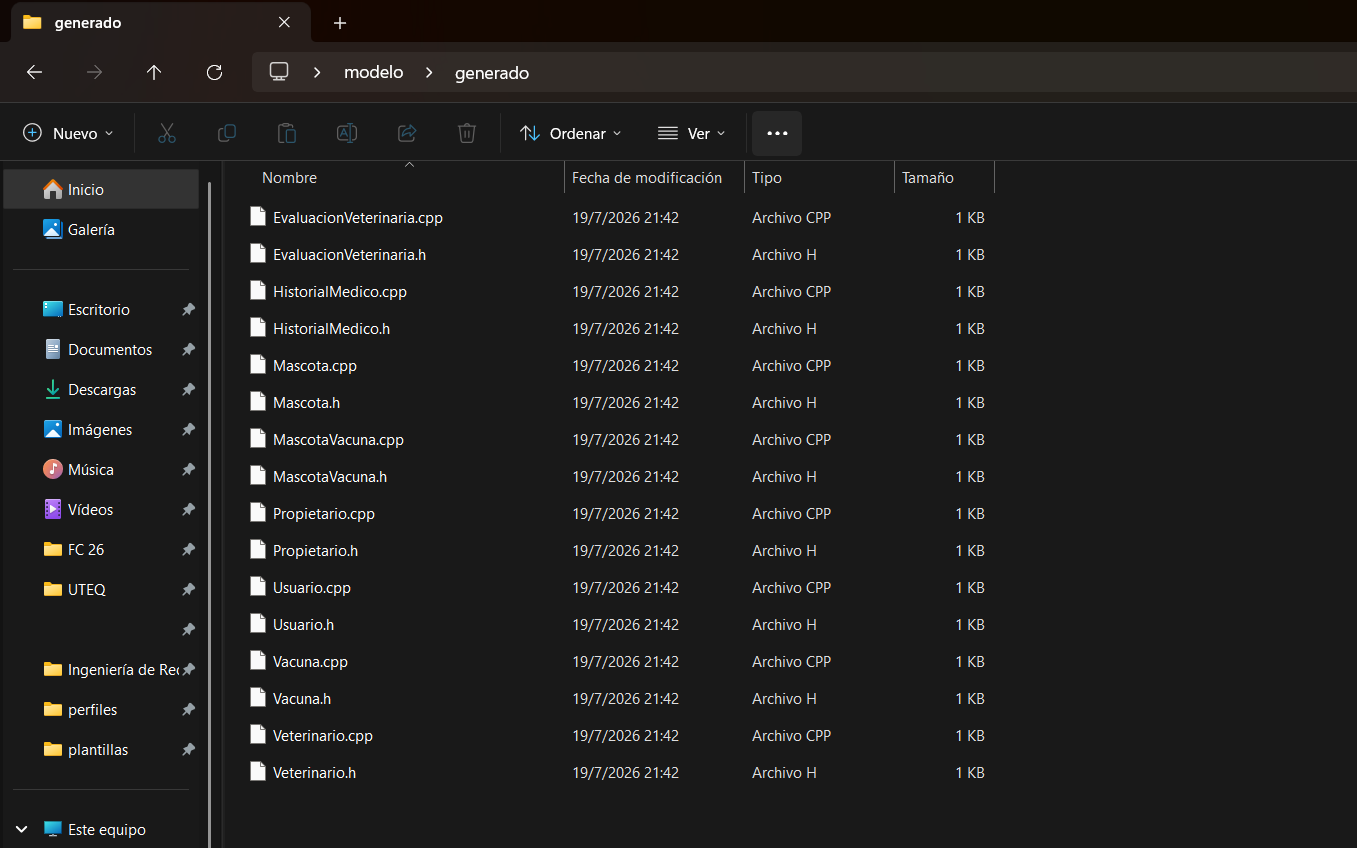
\includegraphics[width=0.55\linewidth]{figuras/arbol_proyecto_generado.png}
		\caption{Árbol de archivos generados en la carpeta \texttt{generado/} a partir del modelo UML en BOUML.}
		\label{fig:arbol_generado}
	\end{figure}
	
	% ============================================================
	% 7. VERIFICACIÓN DEL CÓDIGO GENERADO
	% ============================================================
	\section{Verificación del código generado}
	
	\subsection{Compilación y ejecución}
	El proyecto generado por BOUML se compiló utilizando el compilador \textbf{g++} (MinGW) mediante el siguiente comando, ejecutado sobre la carpeta \textbf{generado/}:
	
	\begin{verbatim}
		g++ Usuario.cpp Propietario.cpp Veterinario.cpp Mascota.cpp
		HistorialMedico.cpp Vacuna.cpp MascotaVacuna.cpp
		EvaluacionVeterinaria.cpp main.cpp -o mundipets_demo
	\end{verbatim}
	
	Como unidad mínima demostrable, se elaboró un archivo \texttt{main.cpp} que instancia un objeto \textit{Propietario} y un objeto \textit{Mascota}, enlaza la asociación entre ambos mediante los punteros generados por BOUML (mascota1.propietarioy propietario1.mascotas), y verifica en tiempo de ejecución la navegación bidireccional de dicha asociación. La compilación finalizó sin errores, generando el ejecutable \texttt{mundipets\_demo.exe}, cuya salida en consola confirma que la relación entre ambas entidades quedó correctamente enlazada en memoria, tal como se muestra en la Figura \ref{fig:ejecucion_demo}.
	
	\begin{figure}[H]
		\centering
		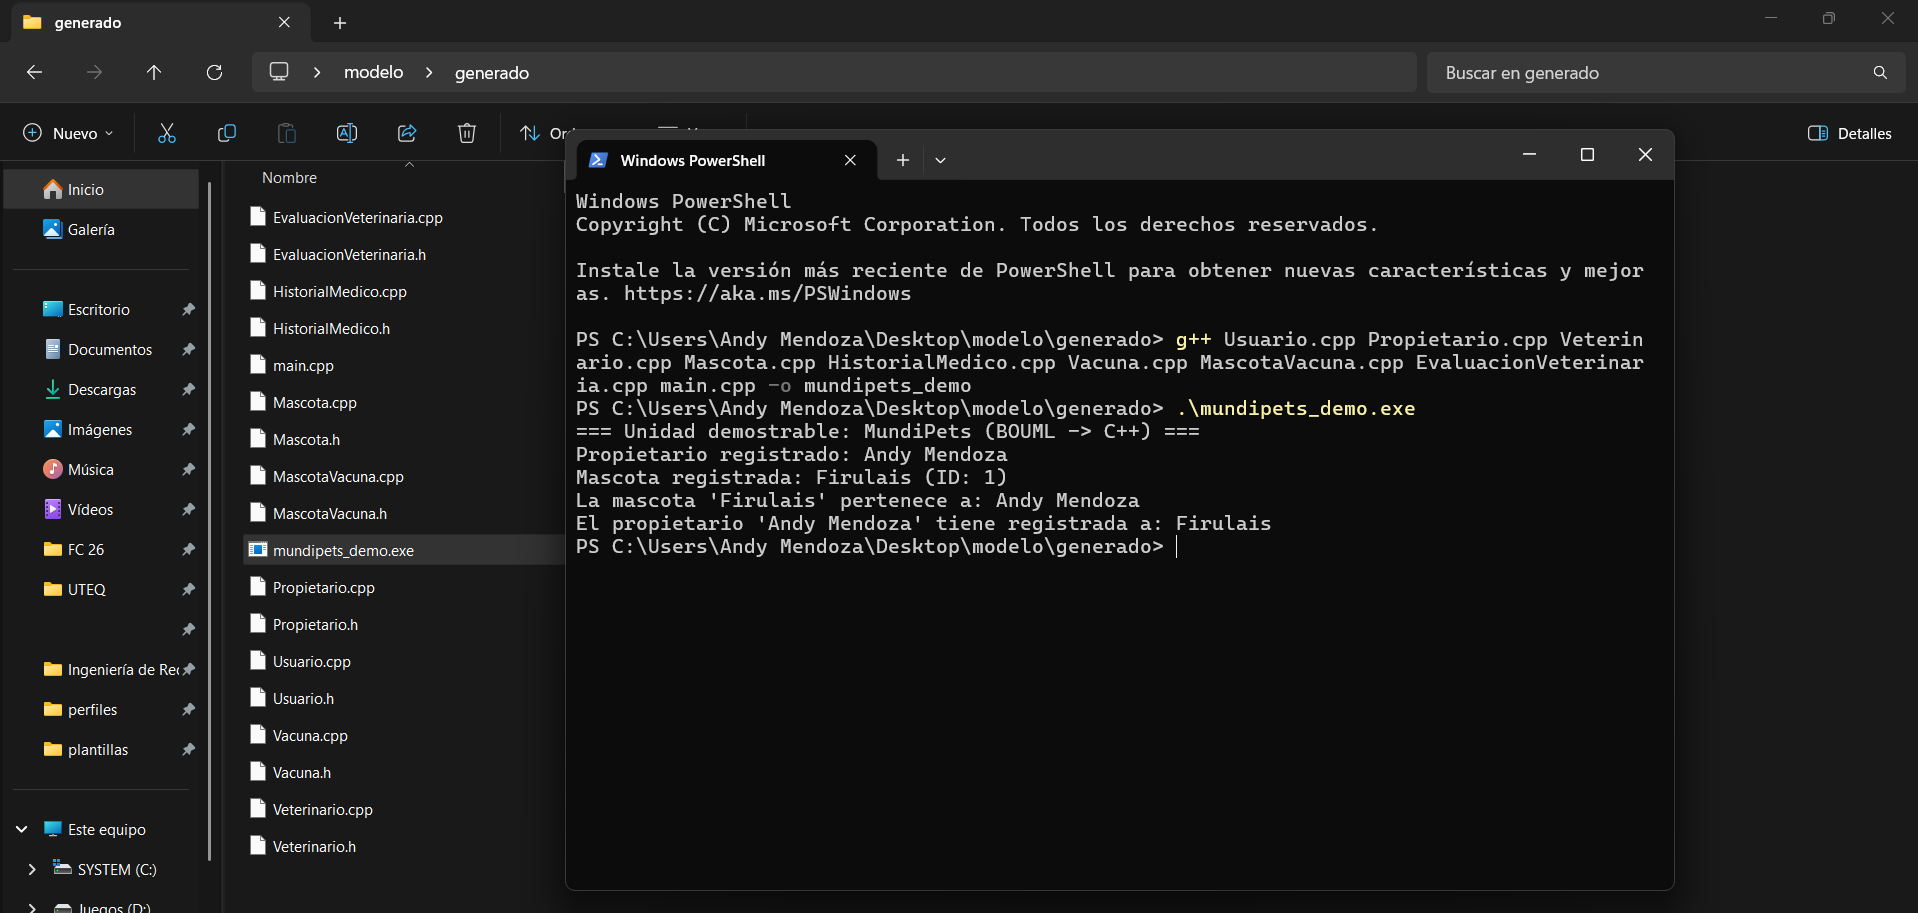
\includegraphics[width=0.62\linewidth]{figuras/ejecucion_demo.png}
		\caption{Salida en consola del ejecutable generado, confirmando la instanciación y asociación correcta de Propietario y Mascota.}
		\label{fig:ejecucion_demo}
	\end{figure}
	
	\subsection{Correspondencia modelo $\to$ código}
	La Tabla \ref{tab:correspondencia} documenta la trazabilidad entre los elementos definidos en el diagrama de clases de origen (Sección 4) y los artefactos concretos que el generador C++ de BOUML produjo en la carpeta generado/.
	
	\begin{table}[H]
		\centering
		\caption{Correspondencia entre elementos del modelo UML y artefactos C++ generados.}
		\label{tab:correspondencia}
		\begin{tabularx}{\linewidth}{|l|X|}
			\hline
			\textbf{Elemento UML} & \textbf{Artefacto C++ generado} \\
			\hline
			Clase Mascota & Mascota.h / Mascota.cpp \\ \hline
			Atributo idMascota (long, público) & Campo público long idMascota; en Mascota.h \\ \hline
			Atributo nombre (string, público) & Campo público string nombre; en Mascota.h \\ \hline
			Generalización Usuario $\to$ Propietario & class Propietario : public Usuario en Propietario.h \\ \hline
			Asociación 1--N Propietario (1) $\leftrightarrow$ Mascota (0..*) & Puntero Propietario * propietario; en Mascota.h, y Mascota * mascotas; en Propietario.h \\ \hline
			Composición Mascota $\blacklozenge$ HistorialMedico (1:1) & Miembro por valor HistorialMedico historial; en Mascota.h \\ \hline
			Asociación 1--N Mascota (1) $\leftrightarrow$ EvaluacionVeterinaria (0..*) & Puntero EvaluacionVeterinaria * evaluaciones; en Mascota.h \\ \hline
			Asociación 1--N Veterinario (1) $\leftrightarrow$ EvaluacionVeterinaria (0..*) & Puntero EvaluacionVeterinaria * evaluacionesRegistradas; en Veterinario.h \\ \hline
			Clase asociativa MascotaVacuna & MascotaVacuna.h / MascotaVacuna.cpp; a diferencia de lo planificado, el generador \textbf{no} produjo ninguna referencia por puntero ni por contenedor \texttt{vector} entre \texttt{Vacuna.h} y \texttt{MascotaVacuna}: el vínculo quedó resuelto únicamente mediante los atributos \texttt{idMascota} e \texttt{idVacuna} (tipo \texttt{long}) declarados dentro de \texttt{MascotaVacuna.h}, a modo de clave foránea, sin navegabilidad por objeto (ver limitación en Sección 7.3) \\ \hline
		\end{tabularx}
	\end{table}
	
	\subsection{Limitaciones detectadas}
	Durante el proceso de generación y verificación se identificaron seis limitaciones concretas del generador C++ de BOUML frente al alcance planificado en la Sección 6.2:
	\begin{itemize}
		\item \textbf{Plantilla de asociación dependiente de un estereotipo vacío.} La plantilla por defecto incluía el marcador de estereotipo entre símbolos de plantilla de tipo. Cuando la asociación no tenía un estereotipo asignado, se sustituía por una cadena vacía dejando los símbolos de apertura y cierre sueltos en el código generado, provocando errores de compilación.
		\item \textbf{Asociaciones sin nombre de rol generadas como atributos anónimos.} Algunas asociaciones quedaron registradas sin un nombre de rol asignado, lo que BOUML tradujo como una declaración de atributo sin identificador, inválida en C++. Estas asociaciones debieron eliminarse individualmente.
		\item \textbf{Contenedores \texttt{vector} no aplicados al entregable final.} Aunque la pestaña C++[5] del generador permite resolver tipos contenedores externos, el equipo optó por conservar la plantilla nativa de puntero simple en todas las asociaciones con multiplicidad múltiple. En consecuencia, el código final (\texttt{Propietario.h}, \texttt{Mascota.h}, \texttt{Veterinario.h}) no contiene ningún \texttt{vector}, y la navegación 1--N declarada en el modelo queda representada de forma incompleta: un puntero simple solo puede apuntar a un elemento a la vez.
		\item \textbf{Clase asociativa MascotaVacuna sin navegabilidad por objeto.} A diferencia de lo previsto, el generador no produjo ningún puntero entre \texttt{Vacuna} y \texttt{MascotaVacuna} (ni viceversa); el vínculo quedó resuelto únicamente mediante los atributos \texttt{idMascota} e \texttt{idVacuna} (tipo \texttt{long}) dentro de \texttt{MascotaVacuna.h}, a modo de clave foránea sin relación de objetos en memoria.
		\item \textbf{Ausencia de métodos de acceso (getters y setters) generados por defecto.} BOUML no genera automáticamente estos métodos para los atributos; requiere definirlos explícitamente. Se optó por exponer como públicos los atributos estrictamente necesarios para la demostración como una simplificación deliberada.
		\item \textbf{Cuerpo de operación generado sin sentencia \texttt{return}.} La operación \texttt{float Mascota::calcularDosisRecomendada()}, incorporada durante el roundtrip (Sección 9), se generó con el cuerpo vacío. El compilador \texttt{g++} advierte \textit{``no return statement in function returning non-void''}; el código compila y enlaza, pero el valor devuelto por esta operación es indefinido hasta que el equipo complete manualmente su lógica de negocio.
	\end{itemize}
	
	% ============================================================
	% 8. CIERRE DEL CICLO (ROUNDTRIP)
	% ============================================================
	\section{Cierre del ciclo (roundtrip)}
	
	\subsection{Cambio aplicado al modelo}
	Para demostrar operativamente la bidireccionalidad y el cierre del ciclo de desarrollo dirigido por modelos (MDD), se planificó y ejecutó una modificación arquitectónica controlada directamente sobre el diseño estructural del subsistema sanitario \cite{GuiaMDD2026}. El cambio consistió en dotar a la entidad central \textit{Mascota} de la capacidad de almacenar características físicas e incorporar comportamiento lógico para el negocio clínico \cite{ERSMundiPets2026}. 
	
	Específicamente, dentro del lienzo de BOUML se incorporó el atributo privado \texttt{pesoKg} con tipo primitivo \texttt{float}, y se añadió la operación pública \texttt{calcularDosisRecomendada()} con tipo de retorno \texttt{float} \cite{BOUMLFeatures2026}. La estructura original de la entidad previa a esta evolución arquitectónica puede observarse detalladamente en el modelo global de la Figura \ref{fig:bouml_clases} \cite{GuiaMDD2026}. Este escenario simula una evolución real de requisitos en el PFC \textit{MundiPets}, permitiendo evaluar la respuesta del motor ante la alteración del metamodelo de origen sin necesidad de reescribir los archivos desde cero \cite{OMG2017UML, OMG2008MOFM2T}.
	
	\begin{figure}[H]
		\centering
		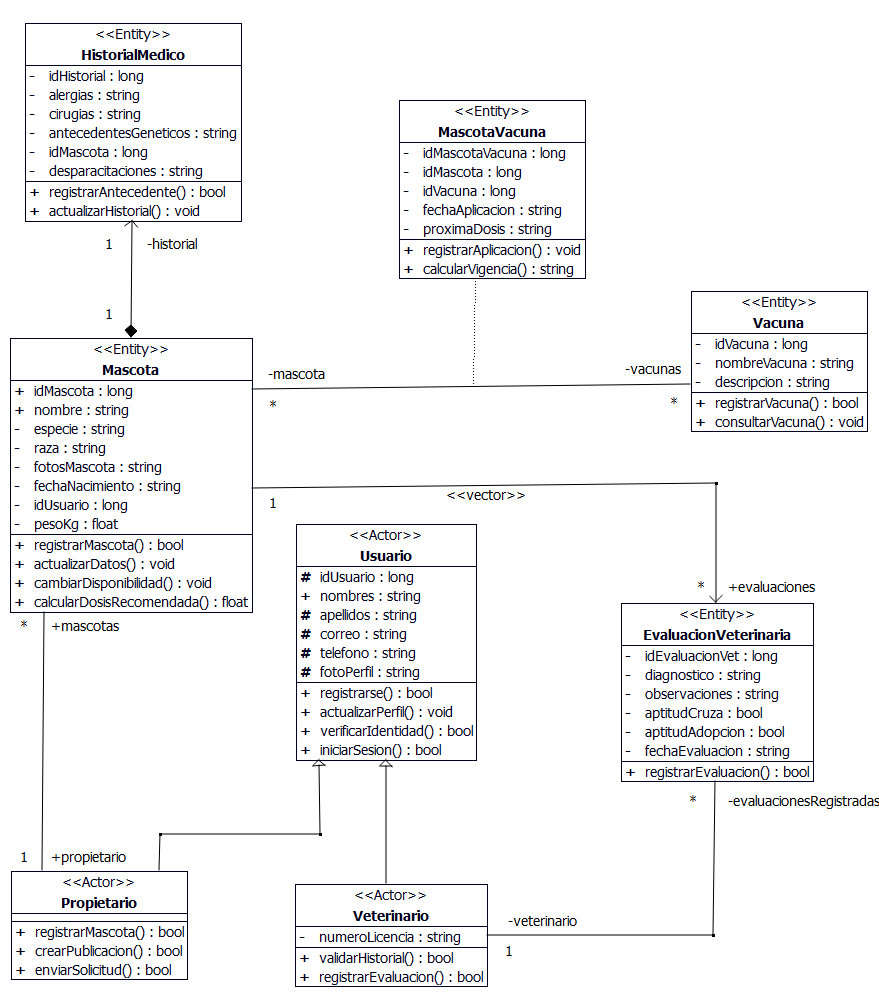
\includegraphics[width=0.75\textwidth]{figuras/despues_modelo.png}
		\caption{Diagrama de clases de la entidad Mascota en BOUML tras incorporar el atributo pesoKg y la operación calcularDosisRecomendada.}
		\label{fig:despues_modelo}
	\end{figure}
	
	\subsection{Evidencia antes/después}
	Una vez aplicado el cambio en el modelo gráfico, la sincronización bidireccional se ejecutó activando el comando específico \textbf{\textit{Roundtrip engineering C++}} desde el menú contextual del paquete de clases en BOUML \cite{BOUMLFeatures2026}. A diferencia de una generación unidireccional simple, este motor lee primero el estado del código físico en el disco para mapear los bloques manuales existentes y, posteriormente, inyecta las nuevas firmas lógicas del Browser de manera consistente \cite{BOUMLFeatures2026, GuiaMDD2026}. Al ingresar al archivo de cabecera \texttt{Mascota.h}, se constató la inserción exitosa de las firmas correspondientes: la variable encapsulada \texttt{float pesoKg;} en la zona privada de la clase y la declaración del método \texttt{float calcularDosisRecomendada();} en la sección pública \cite{BOUMLFeatures2026}.
	
	Un aspecto crítico verificado de forma empírica en este proceso fue el comportamiento del generador frente a la política de \textbf{preservación de bloques protegidos} \cite{BOUMLFeatures2026}. El código manual previamente embebido por el equipo de desarrollo para enlazar las asociaciones de punteros dinámicos no sufrió ninguna alteración ni borrado accidental \cite{Jongeling2022}. El analizador de BOUML aisló las modificaciones estructurales y respetó estrictamente las líneas de código humano situadas entre los marcadores de preservación del entorno, demostrando que el flujo \textit{round-trip} ejecutado es consistente, reproducible y seguro para el desarrollo incremental del backend en C++ \cite{GuiaMDD2026, BOUMLFeatures2026}.
	
	\begin{figure}[H]
		\centering
		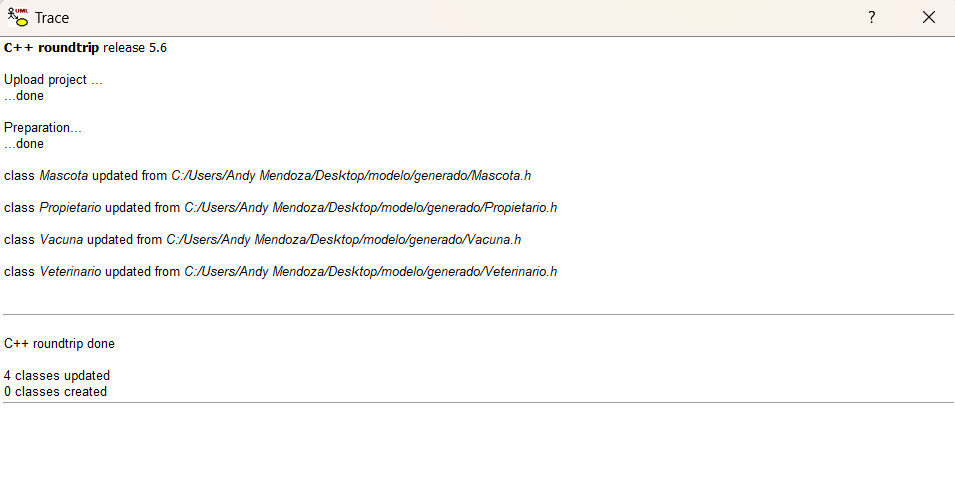
\includegraphics[width=0.5\textwidth]{figuras/diff_codigo.png}
		\caption{Evidencia de la traza de comparación (diff) reflejando la inserción exacta del nuevo atributo y método en Mascota.h respetando los bloques protegidos.}
		\label{fig:diff_codigo}
	\end{figure}
	
	% ============================================================
	% 9. REPARTO DEL TRABAJO Y DOCUMENTACIÓN
	% ============================================================
	\section{Reparto del trabajo}
	Para certificar el cumplimiento pleno de las directrices de trabajo equitativo y asegurar la transparencia en la contribución individual, la distribución de responsabilidades lógicas del proyecto se gobernó bajo un esquema de asignación de fases atómicas \cite{GuiaMDD2026}. Cada integrante del equipo ejecutó sus aportaciones empleando de forma estricta su identidad digital real y cuenta institucional en la plataforma de control de versiones GitHub, vinculando de manera verificable los registros del historial con el desarrollo físico de este reporte y de los componentes de código fuente generados en C++ \cite{GuiaMDD2026}.
	
	La Tabla \ref{tab:reparto_responsabilidades} expone formalmente la distribución de liderazgo técnico y autorías por cada sección consolidada en el informe final.
	
	\begin{table}[H]
		\centering
		\caption{Distribución formal de responsabilidades lógicas por integrante.}
		\label{tab:reparto_responsabilidades}
		\begin{tabularx}{\linewidth}{|c|l|X|}
			\hline
			\textbf{Capítulo} & \textbf{Sección / Fase del Proyecto} & \textbf{Integrante Responsable} \\
			\hline
			\textbf{1} & Marco teórico (Conceptos base y estándares) & Sánchez C. Gary / Chavarría C. Mel \\ \hline
			\textbf{2} & Justificación de la selección de BOUML & Chavarría Cuenca Tahiny Mel \\ \hline
			\textbf{3} & Descripción del subsistema del PFC modelado & Chavarría Cuenca Tahiny Mel \\ \hline
			\textbf{4} & Modelo UML de origen (Lienzo y validación) & Mendoza Párraga Andy Johel \\ \hline
			\textbf{5} & Configuración del generador M2T C++ & Sánchez Cornejo Gary Alberto \\ \hline
			\textbf{6} & Proceso de generación automatizada & Sánchez Cornejo Gary Alberto \\ \hline
			\textbf{7} & Verificación del código generado y pruebas g++ & Sánchez Cornejo Gary Alberto \\ \hline
			\textbf{8} & Cierre del ciclo (\textit{Roundtrip engineering C++}) & Mendoza Párraga Andy Johel \\ \hline
			\textbf{9} & Reparto del trabajo y consistencia Git & Mendoza Párraga Andy Johel \\ \hline
			\textbf{10} & Conclusiones funcionales finales & Equipo H \\
			\hline
		\end{tabularx}
	\end{table}
	
	\subsection{Trazabilidad de contribuciones técnicas e historial en GitHub}
	En concordancia con las restricciones de auditoría académica, las contribuciones técnicas se desarrollaron de manera incremental a través de múltiples confirmaciones de cambio en el servidor. A continuación, se detallan las tareas específicas lideradas por cada estudiante, junto con la dirección URL configurada para auditar el listado completo y cronológico de sus respectivos \textit{commits}:
	
	\begin{itemize}[leftmargin=*]
		\item \textbf{Mendoza Párraga Andy Johel (Titular del PFC)}
		\begin{itemize}
			\item \textit{Foco de contribución técnica:} Diseño, tipificación y normalización del diagrama de clases estructural y casos de uso en el archivo nativo del proyecto; ejecución de controles sintácticos mediante la auditoría \textit{Uml projection}; planeación e inyección interactiva del cambio controlado de requisitos en el modelo (atributo \texttt{pesoKg} y método de dosis) ejecutando el motor de \textit{Roundtrip engineering C++} para verificar el resguardo de bloques protegidos.
			\item \textit{Historial completo de Commits:} \\
			\url{https://github.com/andymendozap03/PFC-MundiPets-MDD-EquipoH-BOUML/commits?author=andymendozap03}
		\end{itemize}
		
		\item \textbf{Sánchez Cornejo Gary Alberto}
		\begin{itemize}
			\item \textit{Foco de contribución técnica:} Fundamentación teórica de las transformaciones M2M/M2T, metamodelos y plantillas del marco conceptual; parametrización global del motor de generación física (rutas de salida, extensiones .h/.cpp, guardas de inclusión) y evaluación de la representación de multiplicidades múltiples mediante punteros simples frente a contenedores \texttt{std::vector} (documentada como limitación en la Sección 7.3); codificación de la unidad demostrable \texttt{main.cpp} y pruebas de compilación nativa con g++.
			\item \textit{Historial completo de Commits:} \\
			\url{https://github.com/andymendozap03/PFC-MundiPets-MDD-EquipoH-BOUML/commits?author=gsanchezc6-beep}
		\end{itemize}
		
		\item \textbf{Chavarría Cuenca Tahiny Mel}
		\begin{itemize}
			\item \textit{Foco de contribución técnica:} Redacción y fundamentación del marco justificativo de la herramienta frente a las restricciones del dominio clínico y la norma de requisitos ISO/IEC/IEEE 29148:2018; diseño de la matriz comparativa de viabilidad contra la alternativa descartada Modelio 5.4.1 y redacción de la sección contextual del ecosistema web de la plataforma.
			\item \textit{Historial completo de Commits:} \\
			\url{https://github.com/andymendozap03/PFC-MundiPets-MDD-EquipoH-BOUML/commits?author=TahinyMel}
		\end{itemize}
	\end{itemize}
	
	\subsection{Log de aportaciones individuales (Insights Contributors)}
	Como evidencia objetiva de la participación continua, balanceada y distribuida a lo largo de todo el ciclo de vida del desarrollo, la Figura \ref{fig:github_contributors} expone la métrica agregada de aportes extraída directamente de la sección de analíticas del repositorio en la nube. 
	
	Se destaca una correlación exacta entre los roles declarados y las métricas del servidor: la estudiante Chavarría lidera la frecuencia transaccional con 16 confirmaciones, el estudiante Mendoza acumula el mayor volumen de adiciones estructurales con 2,190 líneas debido a la inyección del metamodelo y los esqueletos físicos de C++, y el estudiante Sánchez consolida los componentes técnicos complementarios mediante 6 confirmaciones en la etapa final de pruebas.
	
	\begin{figure}[H]
		\centering
		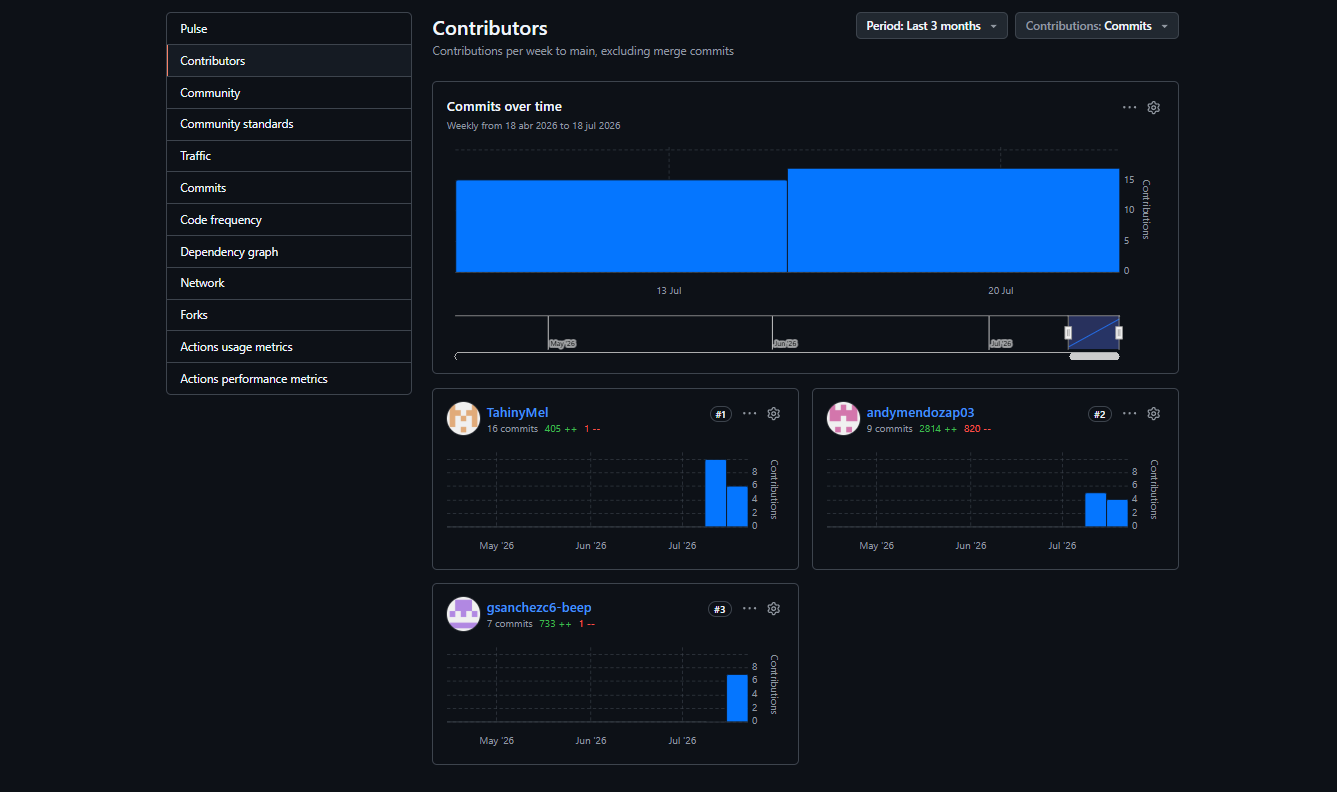
\includegraphics[width=0.75\textwidth]{figuras/github_contributors.png}
		\caption{Métricas de aportes y commits individuales extraídas de la sección Insights/Contributors de GitHub.}
		\label{fig:github_contributors}
	\end{figure}

	% ============================================================
	% 10. CONCLUSIONES
	% ============================================================
	\section{Conclusiones}
	Luego de culminar con todo el ciclo práctico de este proyecto, como equipo pudimos constatar el valor real que tiene el desarrollo guiado por modelos para nuestro sistema MundiPets. La principal ventaja de aplicar este enfoque fue la reducción drástica del trabajo repetitivo en el backend, ya que pudimos automatizar la creación de las ocho clases sanitarias con sus tipos de datos correspondientes. Al dejar que la herramienta se encargue de generar la estructura base, no solo ahorramos tiempo valioso, sino que eliminamos la posibilidad de arrastrar errores humanos al escribir las declaraciones y las herencias nativas en C++. El diseño dejó de ser un simple dibujo decorativo para convertirse en el motor directo de la programación.
	
	El aprendizaje más importante que nos llevamos de esta experiencia es entender cómo funciona el ciclo completo de sincronización bidireccional, conocido como roundtrip engineering. Al principio pensábamos que cualquier cambio en el lienzo destruiría los avances manuales del backend, pero comprobar el funcionamiento de los bloques protegidos de BOUML nos dio una perspectiva completamente diferente. Ver cómo el generador es capaz de inyectar nuevos atributos como el peso de la mascota sin tocar una sola línea de la lógica que programamos a mano nos enseñó que se puede mantener un diseño limpio, ordenado y perfectamente sincronizado a lo largo de todo el ciclo de desarrollo.
	
	Por último, es necesario reconocer que experimentamos limitaciones técnicas importantes durante las pruebas. BOUML es excelente para armar el esqueleto orientado a objetos, pero nos obligó a realizar ajustes manuales debido a que no genera de forma automática los métodos de acceso para los atributos, y sus plantillas por defecto a veces crean código incompleto si las asociaciones no tienen roles definidos. Además, el alcance de la herramienta se limita estrictamente al código lógico de C++, lo que significa que tanto la base de datos como las pantallas de la interfaz gráfica quedan completamente fuera de su control y dependen por entero de nuestro trabajo manual en las siguientes fases del proyecto.
	
	\newpage
	\section{Referencias}
	
	\printbibliography[heading=none]
	
	\newpage
	\section*{Anexos}
	\addcontentsline{toc}{section}{Anexos}
	% ============================================================
	% ANEXO A
	% ============================================================
	\textbf{Anexo A --- Especificación detallada de Requisitos Funcionales del sistema}
	\label{anexo:rf_sanitario}
	
	A continuación, se presenta la especificación atómica detallada de la totalidad de los requisitos funcionales del sistema MundiPets, estructurados bajo los ocho atributos de gestión establecidos por el estándar ISO/IEC/IEEE 29148:2018.
	
	\subsection*{Requisitos Funcionales del Subsistema de Gestión Sanitaria}
	
	\textbf{RF-01 -- Registrar mascota}
	\begin{table}[H]
		\centering\small
		\begin{tabularx}{\linewidth}{|l|X|}
			\hline
			\textbf{Atributo} & \textbf{Valor} \\ \hline
			Identificador & RF-01 \\ \hline
			Nombre & Registrar mascota \\ \hline
			Descripción & El sistema deberá permitir al propietario registrar una mascota ingresando su información general, incluyendo nombre, especie, raza, sexo, edad, estado reproductivo y fotografías para su identificación dentro de la plataforma. \\ \hline
			Prioridad (MoSCoW) & Must \\ \hline
			Fuente / Evidencia & EV-02, EV-03, EV-05, EV-06, EV-07, EV-08 \\ \hline
			Estabilidad & Alta \\ \hline
			Estado & Aprobado \\ \hline
			Criterio de Verificación & Registrar una mascota con datos válidos y comprobar que el perfil queda almacenado y puede consultarse posteriormente. \\ \hline
		\end{tabularx}
	\end{table}
	
	\textbf{RF-02 -- Gestionar historial médico de la mascota}
	\begin{table}[H]
		\centering\small
		\begin{tabularx}{\linewidth}{|l|X|}
			\hline
			\textbf{Atributo} & \textbf{Valor} \\ \hline
			Identificador & RF-02 \\ \hline
			Nombre & Gestionar historial médico de la mascota \\ \hline
			Descripción & El sistema deberá permitir registrar y actualizar el historial médico de una mascota, incluyendo vacunas, desparasitaciones, enfermedades, alergias, cirugías, tratamientos y controles veterinarios. \\ \hline
			Prioridad (MoSCoW) & Must \\ \hline
			Fuente / Evidencia & EV-01, EV-02, EV-03, EV-04, EV-05, EV-06, EV-07 \\ \hline
			Estabilidad & Alta \\ \hline
			Estado & Aprobado \\ \hline
			Criterio de Verificación & Registrar nuevos antecedentes médicos y verificar que aparecen correctamente dentro del historial clínico de la mascota. \\ \hline
		\end{tabularx}
	\end{table}
	
	\textbf{RF-03 -- Consultar perfil completo de una mascota}
	\begin{table}[H]
		\centering\small
		\begin{tabularx}{\linewidth}{|l|X|}
			\hline
			\textbf{Atributo} & \textbf{Valor} \\ \hline
			Identificador & RF-03 \\ \hline
			Nombre & Consultar perfil completo de una mascota \\ \hline
			Descripción & El sistema deberá permitir visualizar el perfil completo de una mascota mostrando su información general, historial médico autorizado, fotografías, comportamiento, vacunas, edad, raza para procesos de adopción o cruza. \\ \hline
			Prioridad (MoSCoW) & Must \\ \hline
			Fuente / Evidencia & EV-02, EV-04, EV-05, EV-06, EV-07, EV-08 \\ \hline
			Estabilidad & Alta \\ \hline
			Estado & Aprobado \\ \hline
			Criterio de Verificación & Consultar una mascota registrada y comprobar que se muestra toda la información autorizada. \\ \hline
		\end{tabularx}
	\end{table}
	
	\textbf{RF-09 -- Validar la información médica de una mascota}
	\begin{table}[H]
		\centering\small
		\begin{tabularx}{\linewidth}{|l|X|}
			\hline
			\textbf{Atributo} & \textbf{Valor} \\ \hline
			Identificador & RF-09 \\ \hline
			Nombre & Validar la información médica de una mascota \\ \hline
			Descripción & El sistema deberá permitir que una veterinaria autorizada valide la información médica registrada de una mascota, indicando que los datos han sido verificados por un profesional. \\ \hline
			Prioridad (MoSCoW) & Must \\ \hline
			Fuente / Evidencia & EV-03, EV-05, EV-07 \\ \hline
			Estabilidad & Alta \\ \hline
			Estado & Aprobado \\ \hline
			Criterio de Verificación & Validar el historial médico de una mascota y comprobar que el sistema muestre el estado de información validada. \\ \hline
		\end{tabularx}
	\end{table}
	
	\textbf{RF-14 -- Gestionar carnet de vacunación}
	\begin{table}[H]
		\centering\small
		\begin{tabularx}{\linewidth}{|l|X|}
			\hline
			\textbf{Atributo} & \textbf{Valor} \\ \hline
			Identificador & RF-14 \\ \hline
			Nombre & Gestionar carnet de vacunación \\ \hline
			Descripción & El sistema deberá permitir registrar, actualizar y consultar el carnet de vacunación de cada mascota, mostrando el historial de vacunas aplicadas, fechas, próximas dosis y su estado de vigencia. \\ \hline
			Prioridad (MoSCoW) & Must \\ \hline
			Fuente / Evidencia & EV-02, EV-03, EV-05, EV-06, EV-07 \\ \hline
			Estabilidad & Alta \\ \hline
			Estado & Aprobado \\ \hline
			Criterio de Verificación & Registrar una vacuna y comprobar que aparezca correctamente en el carnet de vacunación. \\ \hline
		\end{tabularx}
	\end{table}
	
	\textbf{RF-16 -- Gestionar antecedentes genéticos y parentesco de la mascota}
	\begin{table}[H]
		\centering\small
		\begin{tabularx}{\linewidth}{|l|X|}
			\hline
			\textbf{Atributo} & \textbf{Valor} \\ \hline
			Identificador & RF-16 \\ \hline
			Nombre & Gestionar antecedentes genéticos y parentesco de la mascota \\ \hline
			Descripción & El sistema deberá permitir registrar y consultar los antecedentes genéticos y el grado de parentesco de una mascota, incluyendo información sobre enfermedades hereditarias y linaje para apoyar los procesos de cruza responsable y la evaluación de compatibilidad. \\ \hline
			Prioridad (MoSCoW) & Must \\ \hline
			Fuente / Evidencia & EV-01, EV-03, EV-05, EV-07 \\ \hline
			Estabilidad & Alta \\ \hline
			Estado & Aprobado \\ \hline
			Criterio de Verificación & Registrar antecedentes genéticos para una mascota y comprobar que la información quede almacenada. \\ \hline
		\end{tabularx}
	\end{table}
	
	\subsection*{Requisitos Funcionales Transaccionales y de Soporte}
	
	\textbf{RF-04 -- Buscar y filtrar mascotas}
	\begin{table}[H]
		\centering\small
		\begin{tabularx}{\linewidth}{|l|X|}
			\hline
			\textbf{Atributo} & \textbf{Valor} \\ \hline
			Identificador & RF-04 \\ \hline
			Nombre & Buscar y filtrar mascotas \\ \hline
			Descripción & El sistema deberá permitir buscar mascotas aplicando filtros como especie, raza, edad, ubicación, estado de salud y disponibilidad para adopción o cruza. \\ \hline
			Prioridad (MoSCoW) & Should \\ \hline
			Fuente / Evidencia & EV-07, EV-08 \\ \hline
			Estabilidad & Media \\ \hline
			Estado & Aprobado \\ \hline
			Criterio de Verificación & Aplicar diferentes filtros y comprobar que los resultados corresponden con los criterios seleccionados. \\ \hline
		\end{tabularx}
	\end{table}
	
	\textbf{RF-05 -- Gestionar solicitudes de adopción}
	\begin{table}[H]
		\centering\small
		\begin{tabularx}{\linewidth}{|l|X|}
			\hline
			\textbf{Atributo} & \textbf{Valor} \\ \hline
			Identificador & RF-05 \\ \hline
			Nombre & Gestionar solicitudes de adopción \\ \hline
			Descripción & El sistema deberá permitir que un usuario interesado envíe solicitudes de adopción y que el propietario pueda aceptarlas o rechazarlas después de revisar la información del solicitante. \\ \hline
			Prioridad (MoSCoW) & Must \\ \hline
			Fuente / Evidencia & EV-01, EV-02, EV-03, EV-05, EV-06, EV-08 \\ \hline
			Estabilidad & Alta \\ \hline
			Estado & Aprobado \\ \hline
			Criterio de Verificación & Registrar una solicitud y comprobar que el propietario puede gestionarla correctamente. \\ \hline
		\end{tabularx}
	\end{table}
	
	\textbf{RF-06 -- Evaluar compatibilidad entre mascotas para cruza}
	\begin{table}[H]
		\centering\small
		\begin{tabularx}{\linewidth}{|l|X|}
			\hline
			\textbf{Atributo} & \textbf{Valor} \\ \hline
			Identificador & RF-06 \\ \hline
			Nombre & Evaluar compatibilidad entre mascotas para cruza \\ \hline
			Descripción & El sistema deberá evaluar la compatibilidad entre dos mascotas registradas para procesos de cruza considerando la raza, edad, estado de salud, antecedentes genéticos, parentesco, comportamiento e historial médico, mostrando al usuario el resultado obtenido para apoyar la toma de decisiones. \\ \hline
			Prioridad (MoSCoW) & Must \\ \hline
			Fuente / Evidencia & EV-01, EV-02, EV-03, EV-04, EV-05, EV-06, EV-07, EV-08 \\ \hline
			Estabilidad & Alta \\ \hline
			Estado & Aprobado \\ \hline
			Criterio de Verificación & Seleccionar dos mascotas y comprobar que el sistema presenta la información de compatibilidad. \\ \hline
		\end{tabularx}
	\end{table}
	
	\textbf{RF-07 -- Sistema de mensajería entre usuarios}
	\begin{table}[H]
		\centering\small
		\begin{tabularx}{\linewidth}{|l|X|}
			\hline
			\textbf{Atributo} & \textbf{Valor} \\ \hline
			Identificador & RF-07 \\ \hline
			Nombre & Sistema de mensajería entre usuarios \\ \hline
			Descripción & El sistema deberá habilitar un canal de comunicación entre dos usuarios registrados cuando exista un proceso de adopción o cruza activo entre ellos. \\ \hline
			Prioridad (MoSCoW) & Could \\ \hline
			Fuente / Evidencia & EV-02, EV-07, EV-08 \\ \hline
			Estabilidad & Media \\ \hline
			Estado & Aprobado \\ \hline
			Criterio de Verificación & Enviar un mensaje entre dos usuarios autorizados y verificar que ambos puedan visualizarlo. \\ \hline
		\end{tabularx}
	\end{table}
	
	\textbf{RF-08 -- Gestionar solicitudes de cruza}
	\begin{table}[H]
		\centering\small
		\begin{tabularx}{\linewidth}{|l|X|}
			\hline
			\textbf{Atributo} & \textbf{Valor} \\ \hline
			Identificador & RF-08 \\ \hline
			Nombre & Gestionar solicitudes de cruza \\ \hline
			Descripción & El sistema deberá permitir que los propietarios soliciten procesos de cruza entre mascotas y que el propietario de la otra mascota pueda aceptar o rechazar la solicitud con base en la información disponible. \\ \hline
			Prioridad (MoSCoW) & Must \\ \hline
			Fuente / Evidencia & EV-01, EV-02, EV-03, EV-05, EV-06, EV-07 \\ \hline
			Estabilidad & Alta \\ \hline
			Estado & Aprobado \\ \hline
			Criterio de Verificación & Registrar una solicitud de cruza y verificar que el propietario receptor pueda gestionarla. \\ \hline
		\end{tabularx}
	\end{table}
	
	\textbf{RF-10 -- Gestionar recordatorios de controles preventivos}
	\begin{table}[H]
		\centering\small
		\begin{tabularx}{\linewidth}{|l|X|}
			\hline
			\textbf{Atributo} & \textbf{Valor} \\ \hline
			Identificador & RF-10 \\ \hline
			Nombre & Gestionar recordatorios de controles preventivos \\ \hline
			Descripción & El sistema deberá enviar un recordatorio al propietario de la mascota antes de la fecha programada de una cita veterinaria y registrar el envío de la notificación. \\ \hline
			Prioridad (MoSCoW) & Should \\ \hline
			Fuente / Evidencia & EV-02, EV-04, EV-06 \\ \hline
			Estabilidad & Media \\ \hline
			Estado & Aprobado \\ \hline
			Criterio de Verificación & Configurar una alerta de control próximo y verificar el registro de envío de la notificación. \\ \hline
		\end{tabularx}
	\end{table}
	
	\textbf{RF-11 -- Administrar la privacidad de la información}
	\begin{table}[H]
		\centering\small
		\begin{tabularx}{\linewidth}{|l|X|}
			\hline
			\textbf{Atributo} & \textbf{Valor} \\ \hline
			Identificador & RF-11 \\ \hline
			Nombre & Administrar la privacidad de la información \\ \hline
			Descripción & El sistema deberá permitir que el propietario determine qué información de su mascota y de su perfil podrá ser visualizada por otros usuarios, protegiendo los datos considerados sensibles. \\ \hline
			Prioridad (MoSCoW) & Must \\ \hline
			Fuente / Evidencia & EV-02, EV-05, EV-06, EV-07, EV-08 \\ \hline
			Estabilidad & Alta \\ \hline
			Estado & Aprobado \\ \hline
			Criterio de Verificación & Modificar la configuración de privacidad y comprobar que los datos restringidos dejen de ser visibles. \\ \hline
		\end{tabularx}
	\end{table}
	
	\textbf{RF-12 -- Verificar la identidad de los usuarios}
	\begin{table}[H]
		\centering\small
		\begin{tabularx}{\linewidth}{|l|X|}
			\hline
			\textbf{Atributo} & \textbf{Valor} \\ \hline
			Identificador & RF-12 \\ \hline
			Nombre & Verificar la identidad de los usuarios \\ \hline
			Descripción & El sistema deberá validar la información obligatoria proporcionada por el usuario antes de aprobar el proceso de verificación de identidad. \\ \hline
			Prioridad (MoSCoW) & Must \\ \hline
			Fuente / Evidencia & EV-01, EV-03, EV-07, EV-08 \\ \hline
			Estabilidad & Alta \\ \hline
			Estado & Aprobado \\ \hline
			Criterio de Verificación & Registrar un usuario con la documentación requerida y comprobar que el sistema cambie el estado de verificación. \\ \hline
		\end{tabularx}
	\end{table}
	
	\textbf{RF-13 -- Registrar publicaciones de mascotas}
	\begin{table}[H]
		\centering\small
		\begin{tabularx}{\linewidth}{|l|X|}
			\hline
			\textbf{Atributo} & \textbf{Valor} \\ \hline
			Identificador & RF-13 \\ \hline
			Nombre & Registrar publicaciones de mascotas \\ \hline
			Descripción & El sistema deberá permitir al propietario publicar una mascota indicando si estará disponible para adopción, cruza o ambas opciones, incluyendo toda la información autorizada del perfil de la mascota. \\ \hline
			Prioridad (MoSCoW) & Must \\ \hline
			Fuente / Evidencia & EV-01, EV-02, EV-04, EV-06, EV-07, EV-08 \\ \hline
			Estabilidad & Alta \\ \hline
			Estado & Aprobado \\ \hline
			Criterio de Verificación & Publicar una mascota y comprobar que aparezca correctamente en el listado seleccionado. \\ \hline
		\end{tabularx}
	\end{table}
	
	\textbf{RF-15 -- Consultar el historial de procesos de adopción y cruza}
	\begin{table}[H]
		\centering\small
		\begin{tabularx}{\linewidth}{|l|X|}
			\hline
			\textbf{Atributo} & \textbf{Valor} \\ \hline
			Identificador & RF-15 \\ \hline
			Nombre & Consultar el historial de procesos de adopción y cruza \\ \hline
			Descripción & El sistema deberá permitir al propietario consultar el historial de solicitudes y procesos de adopción y cruza asociados a sus mascotas, incluyendo su estado y fecha de realización. \\ \hline
			Prioridad (MoSCoW) & Could \\ \hline
			Fuente / Evidencia & EV-01, EV-02, EV-04, EV-06 \\ \hline
			Estabilidad & Media \\ \hline
			Estado & Aprobado \\ \hline
			Criterio de Verificación & Acceder al panel histórico del propietario y verificar las trazas y estados de solicitudes pasadas. \\ \hline
		\end{tabularx}
	\end{table}
	
	\textbf{RF-17 -- Validar imágenes de publicaciones}
	\begin{table}[H]
		\centering\small
		\begin{tabularx}{\linewidth}{|l|X|}
			\hline
			\textbf{Atributo} & \textbf{Valor} \\ \hline
			Identificador & RF-17 \\ \hline
			Nombre & Validar imágenes de publicaciones \\ \hline
			Descripción & El sistema deberá validar las imágenes cargadas por los usuarios verificando que cumplan con las políticas de contenido establecidas por la plataforma antes de permitir su publicación. \\ \hline
			Prioridad (MoSCoW) & Should \\ \hline
			Fuente / Evidencia & EV-01, EV-03, EV-05, EV-07, EV-08 \\ \hline
			Estabilidad & Media \\ \hline
			Estado & Aprobado \\ \hline
			Criterio de Verificación & Cargar archivos multimedia conformes y no conformes, y comprobar la respuesta del módulo de validación. \\ \hline
		\end{tabularx}
	\end{table}
	
	\newpage
	\textbf{Anexo B --- Estructura del repositorio GitHub}
	\label{anexo:arbol_repositorio}
	
	A continuación, se detalla la organización física y jerárquica de la raíz del repositorio oficial en GitHub:
	
	\begin{verbatim}
		PFC-MundiPets-MDD-EquipoH-BOUML/
		|   README.md
		|
		|-- aportes_individuales/             (Aportes conceptuales y teóricos)
		|   |-- CHAVARRIA CUENCA TAHINY MEL
		|   |       Aporte_MelChavarria.pdf
		|   |       referencias.bib
		|   |
		|   |-- MENDOZA PARRAGA ANDY JOHEL
		|   |       AndyMendoza_Aporte.pdf
		|   |       referencias.bib
		|   |
		|   \-- SANCHEZ CORNEJO GARY ALBERTO
		|           MarcoTeorico_ERS.pdf
		|           Referencias_MarcoTeorico.bib
		|
		|-- docs/                             (Soporte físico del manuscrito)
		|   |   informe.pdf
		|   |   informe.tex
		|   |   referencias.bib
		|   |
		|   \-- figuras/                      (Diagramas y capturas del informe)
		|
		|-- evidencias/
		|   \-- capturas/                     (Capturas del proceso completo)
		|
		|-- exposicion/                       (Sustentación académica)
		|   \-- DiapositivasBOUML.pdf
		|
		|-- generado/                         (16 archivos del backend de C++)
		|   |   *.h / *.cpp                   (8 clases generadas estructuralmente)
		|   |   main.cpp                      (Unidad demostrable del sistema)
		|   \-- mundipets_demo.exe            (Ejecutable de prueba g++)
		|
		|-- modelo/                           (Proyecto nativo del entorno CASE)
		|   |   128130.diagram                (Lienzo de Casos de Uso)
		|   |   134658.diagram                (Lienzo de Clases de origen)
		|   |   cpp_includes
		|   |   generation_settings
		|   |   modelo.prj                    (Árbol del metamodelo en BOUML)
		|   |   stereotypes
		|   |   tools
		|   |
		|   \-- perfiles/                     (Extensiones del metamodelo)
		|           stereotypes
		|
		\-- plantillas/                       (Parametrización del motor M2T)
		generation_settings
	\end{verbatim}
	
	\newpage
	\textbf{Anexo C --- Tabla de mapeo extensa (Metamodelo UML a C++)}
	\label{anexo:tabla_mapeo_extensa}
	
	La siguiente matriz documenta la correspondencia semántica y sintáctica detallada entre los elementos conceptuales del diagrama de clases de origen diseñado en BOUML y las estructuras de código fuente físicas resultantes en lenguaje C++ tras la ejecución del motor de ingeniería directa:
	
	\begin{longtable}{|p{3.5cm}|p{3.5cm}|p{4.2cm}|p{3.8cm}|}
		\hline
		\textbf{Elemento UML Origen} & \textbf{Estereotipo / Tipo} & \textbf{Estructura Física C++} & \textbf{Archivo de Salida} \\
		\hline
		\endfirsthead
		\hline
		\textbf{Elemento UML Origen} & \textbf{Estereotipo / Tipo} & \textbf{Estructura Física C++} & \textbf{Archivo de Salida} \\
		\hline
		\endhead
		\hline
		\footnoterule
		\endfoot
		\hline
		\endlastfoot
		Clase Usuario & <<Actor>> & class Usuario \{ & Usuario.h \\ \hline
		Atributo idUsuario & protected long & protected: long idUsuario; & Usuario.h \\ \hline
		Atributo contrasena & private string & private: string contrasena; & Usuario.h \\ \hline
		Operación iniciarSesion() & public bool & bool iniciarSesion(); & Usuario.h / .cpp \\ \hline
		
		Clase Propietario & <<Actor>> & class Propietario : public Usuario \{ & Propietario.h \\ \hline
		Relación Generalización & Herencia Nativa & : public Usuario & Propietario.h \\ \hline
		Asociación Propietario $\leftrightarrow$ Mascota & Cardinalidad 0..* & Mascota * mascotas; (puntero simple, plantilla nativa) & Propietario.h \\ \hline
		
		Clase Veterinario & <<Actor>> & class Veterinario : public Usuario \{ & Veterinario.h \\ \hline
		Atributo numLicencia & private string & private: string numLicencia; & Veterinario.h \\ \hline
		
		Clase Mascota & <<Entity>> & class Mascota \{ & Mascota.h \\ \hline
		Atributo idMascota & public long & public: long idMascota; & Mascota.h \\ \hline
		Atributo nombre & public string & public: string nombre; & Mascota.h \\ \hline
		Atributo pesoKg (Mutación) & private float & private: float pesoKg; & Mascota.h \\ \hline
		Operación calcularDosis() & public float & float calcularDosisRecomendada(); & Mascota.h / .cpp \\ \hline
		Asociación Mascota $\leftrightarrow$ Propietario & Cardinalidad 1 & Propietario* propietario; & Mascota.h \\ \hline
		
		Clase HistorialMedico & <<Entity>> & class HistorialMedico \{ & HistorialMedico.h \\ \hline
		Composición Mascota $\blacklozenge$ Historial & Cardinalidad 1:1 (Por Valor) & HistorialMedico historial; & Mascota.h \\ \hline
		
		Clase Vacuna & <<Entity>> & class Vacuna \{ & Vacuna.h \\ \hline
		Atributo idVacuna & private long & private: long idVacuna; & Vacuna.h \\ \hline
		
		Clase Asociativa MascotaVacuna & <<Entity>> M:N & class MascotaVacuna \{ & MascotaVacuna.h \\ \hline
		Vínculo MascotaVacuna $\to$ Mascota & \textbf{No generado como referencia por objeto} & long idMascota; (clave foránea por valor, sin puntero \texttt{Mascota*}) & MascotaVacuna.h \\ \hline
		Vínculo MascotaVacuna $\to$ Vacuna & \textbf{No generado como referencia por objeto} & long idVacuna; (clave foránea por valor, sin puntero \texttt{Vacuna*}) & MascotaVacuna.h \\ \hline
		Asociación Vacuna $\leftrightarrow$ MascotaVacuna & Cardinalidad Múltiple & \textbf{Sin representación en el código generado.} Vacuna.h no declara ningún miembro que referencie a MascotaVacuna & Vacuna.h \\ \hline
		
		Clase EvaluacionVeterinaria & <<Entity>> & class EvaluacionVeterinaria \{ & EvaluacionVeterinaria.h \\ \hline
		Asociación Mascota $\to$ Evaluación & Unidireccional 0..* & EvaluacionVeterinaria * evaluaciones; (puntero simple, plantilla nativa) & Mascota.h \\ \hline
		Asociación Veterinario $\leftrightarrow$ Evaluación & Bidireccional Simple 0..* & EvaluacionVeterinaria * evaluacionesRegistradas; (puntero simple, plantilla nativa) & Veterinario.h \\ \hline
	\end{longtable}
	
	\newpage
	\textbf{Anexo D --- Fragmentos de código fuente representativos}
	\label{anexo:codigo_generado}
	
	A continuación se exponen las definiciones de las estructuras físicas mapeadas e instanciadas por el motor de generación M2T de BOUML para las clases del subsistema sanitario de MundiPets:
	
	\textbf{1. Clase EvaluacionVeterinaria}
	\begin{lstlisting}[caption={Clase EvaluacionVeterinaria (EvaluacionVeterinaria.h).}]
		#ifndef _EVALUACIONVETERINARIA_H
		#define _EVALUACIONVETERINARIA_H
		
		#include <string>
		using namespace std;
		
		class Veterinario;
		
		// <<Entity>>
		class EvaluacionVeterinaria {
			private:
			long idEvaluacionVet;
			string diagnostico;
			string observaciones;
			bool aptitudCruza;
			bool aptitudAdopcion;
			string fechaEvaluacion;
			
			public:
			bool registrarEvaluacion();
			
			private:
			Veterinario * veterinario;
		};
		#endif
	\end{lstlisting}
	
	\textbf{2. Clase HistorialMedico}
	\begin{lstlisting}[caption={Clase HistorialMedico (HistorialMedico.h).}]
		#ifndef _HISTORIALMEDICO_H
		#define _HISTORIALMEDICO_H
		
		#include <string>
		using namespace std;
		
		// <<Entity>>
		class HistorialMedico {
			private:
			long idHistorial;
			string alergias;
			string cirugias;
			string antecedentesGeneticos;
			long idMascota;
			string desparacitaciones;
			
			public:
			bool registrarAntecedente();
			void actualizarHistorial();
		};
		#endif
	\end{lstlisting}
	\newpage
	
	\textbf{3. Clase Mascota}
	\begin{lstlisting}[caption={Clase Mascota (Mascota.h).}]
		#ifndef _MASCOTA_H
		#define _MASCOTA_H
		
		#include <string>
		using namespace std;
		#include "HistorialMedico.h"
		
		class EvaluacionVeterinaria;
		class Propietario;
		class Vacuna;
		
		// <<Entity>>
		class Mascota {
			public:
			long idMascota;
			string nombre;
			
			private:
			string especie;
			string raza;
			string fotosMascota;
			string fechaNacimiento;
			long idUsuario;
			HistorialMedico historial;
			
			public:
			EvaluacionVeterinaria * evaluaciones;
			bool registrarMascota();
			void actualizarDatos();
			void cambiarDisponibilidad();
			Propietario * propietario;
			
			private:
			Vacuna * vacunas;
			float pesoKg;
			
			public:
			float calcularDosisRecomendada();
		};
		#endif
	\end{lstlisting}
	
	\textbf{4. Clase MascotaVacuna}
	\begin{lstlisting}[caption={Clase MascotaVacuna (MascotaVacuna.h).}]
		#ifndef _MASCOTAVACUNA_H
		#define _MASCOTAVACUNA_H
		
		#include <string>
		using namespace std;
		
		// <<Entity>>
		class MascotaVacuna {
			private:
			long idMascotaVacuna;
			long idMascota;
			long idVacuna;
			string fechaAplicacion;
			string proximaDosis;
			
			public:
			void registrarAplicacion();
			string calcularVigencia();
		};
		#endif
	\end{lstlisting}
	
	\textbf{5. Clase Propietario}
	\begin{lstlisting}[caption={Clase Propietario (Propietario.h).}]
		#ifndef _PROPIETARIO_H
		#define _PROPIETARIO_H
		
		#include "Usuario.h"
		
		class Mascota;
		
		// <<Actor>>
		class Propietario : public Usuario {
			public:
			bool registrarMascota();
			bool crearPublicacion();
			bool enviarSolicitud();
			Mascota * mascotas;
		};
		#endif
	\end{lstlisting}
	
	\textbf{6. Clase Usuario}
	\begin{lstlisting}[caption={Clase Usuario (Usuario.h).}]
		#ifndef _USUARIO_H
		#define _USUARIO_H
		
		#include <string>
		using namespace std;
		
		// <<Actor>>
		class Usuario {
			protected:
			long idUsuario;
			
			public:
			string nombres;
			
			protected:
			string apellidos;
			string correo;
			string telefono;
			string fotoPerfil;
			
			public:
			bool registrarse();
			void actualizarPerfil();
			bool verificarIdentidad();
			bool iniciarSesion();
		};
		#endif
	\end{lstlisting}
	
	\newpage
	\textbf{7. Clase Vacuna}
	\begin{lstlisting}[caption={Clase Vacuna (Vacuna.h).}]
		#ifndef _VACUNA_H
		#define _VACUNA_H
		
		#include <string>
		using namespace std;
		
		class Mascota;
		
		// <<Entity>>
		class Vacuna {
			private:
			long idVacuna;
			string nombreVacuna;
			string descripcion;
			
			public:
			bool registrarVacuna();
			void consultarVacuna();
			
			private:
			Mascota * mascota;
		};
		#endif
	\end{lstlisting}
	
	\textbf{8. Clase Veterinario}
	\begin{lstlisting}[caption={Clase Veterinario (Veterinario.h).}]
		#ifndef _VETERINARIO_H
		#define _VETERINARIO_H
		
		#include "Usuario.h"
		#include <string>
		using namespace std;
		
		class EvaluacionVeterinaria;
		
		// <<Actor>>
		class Veterinario : public Usuario {
			private:
			string numeroLicencia;
			
			public:
			bool validarHistorial();
			bool registrarEvaluacion();
			
			private:
			EvaluacionVeterinaria * evaluacionesRegistradas;
		};
		#endif
	\end{lstlisting}
	
	\newpage
	\textbf{Anexo E --- Instrucciones detalladas de reproducibilidad}
	\label{anexo:reproducibilidad}
	
	Para reproducir de forma íntegra el ciclo completo de desarrollo guiado por modelos (MDD) y la compilación del reporte técnico a partir de los artefactos del repositorio oficial:
	
	\begin{enumerate}[leftmargin=*]
		\item \textbf{Clonar el repositorio institucional:} Abrir una terminal de comandos y ejecutar la descarga del repositorio git mediante la instrucción: \\
		\textit{git clone https://github.com/andymendozap03/PFC-MundiPets-MDD-EquipoH-BOUML.git}
		
		\item \textbf{Cargar el proyecto estructural en el entorno CASE:} Iniciar la herramienta BOUML (versión 7.11 patch 4 o superior) y abrir el archivo maestro de configuración del metamodelo situado en la ruta: \\
		\texttt{modelo/modelo.prj}
		
		\item \textbf{Ejecutar la transformación automática Modelo-a-Texto (M2T):} Dentro del explorador de proyectos de BOUML, hacer clic derecho sobre el paquete raíz \textit{modelo}, navegar hacia el menú interactivo \texttt{Generate} y seleccionar la opción \texttt{C++}. El sistema inyectará automáticamente los dieciséis archivos de cabecera e implementación en el directorio físico \texttt{generado/}, aplicando las directivas parametrizadas y resguardando los bloques protegidos.
		
		\item \textbf{Compilar la unidad demostrable del backend:} Acceder mediante la consola de comandos a la carpeta \texttt{generado/} y ejecutar el compilador nativo GCC (g++) para enlazar las clases y el punto de entrada principal mediante la instrucción: \\
		\textit{g++ Usuario.cpp Propietario.cpp Veterinario.cpp Mascota.cpp HistorialMedico.cpp Vacuna.cpp MascotaVacuna.cpp EvaluacionVeterinaria.cpp main.cpp -o mundipets\_demo}
		
		\item \textbf{Ejecutar la unidad demostrable:} Una vez finalizada la compilación de forma exitosa sin advertencias, inicializar el archivo ejecutable resultante en el entorno local para validar la navegación de asociaciones en consola mediante la instrucción: \\
		\textit{.\textbackslash mundipets\_demo.exe}
		
		\item \textbf{Compilar de forma nativa este informe técnico:} En caso de requerir la regeneración física de este documento PDF desde el código fuente, situarse en el directorio \texttt{docs/} y ejecutar secuencialmente las directivas de automatización: \\
		\texttt{pdflatex informe.tex} \\
		\texttt{biber informe} \\
		\texttt{pdflatex informe.tex} (ejecutar dos veces adicionales para estabilizar las referencias cruzadas y los índices).
	\end{enumerate}
	
	
\end{document}